\documentclass[../Main.tex]{subfiles}
\begin{document}
\chapter{Deep Learning}

\intro{
    The modern term “deep learning” goes beyond the neuroscientific perspectiv on the current breed of machine
    learning models. It appeals to a more general principle of learning multiple levels of composition,
    which can be applied in machine learning frameworks that are not necessarily neurally inspired.
}

\begin{figure}[H]
    \centering
    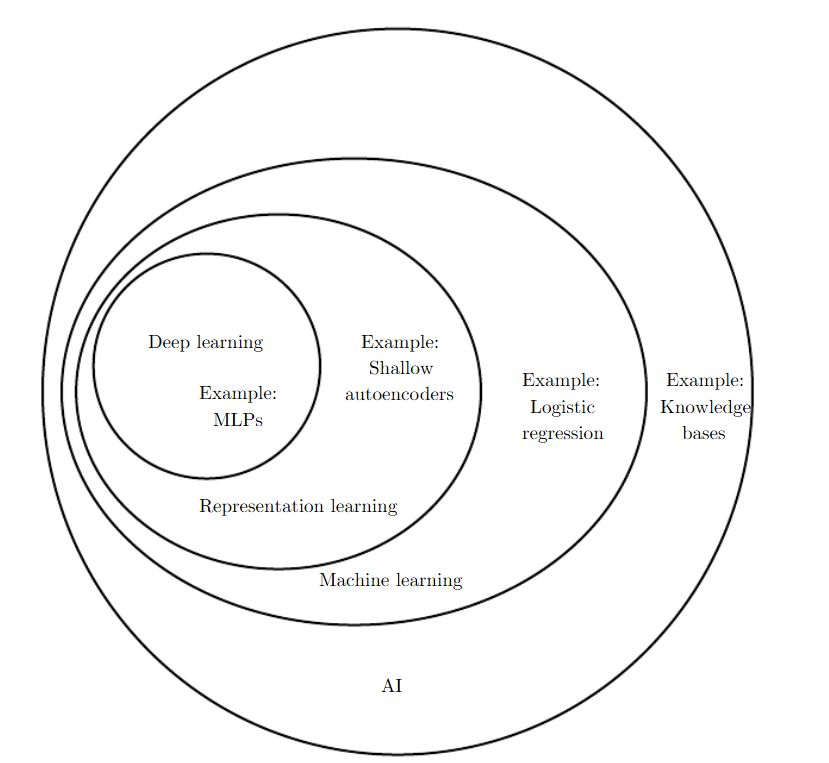
\includegraphics[width=0.75\linewidth]{Images/deepl-venn.png}
    \caption{A Venn diagram showing how deep learning is a kind of representation learning, which is in turn a kind of machine learning, 
    which is used for many but not all approaches to AI. Each section of the Venn diagram includes an example of an AI technology}
\end{figure}

\section{Differences to standard statistical learning methods}
\begin{enumerate}
    \item No manual feature extraction
    \item Arbitarily Complex Models
    \item No Feature Engineering
    \item Flexible Models
\end{enumerate}

\subsection{Reasons for increasing popularity}
\begin{itemize}
    \item Bigger datasets due to increasing digitalization
    \item Increasing Model Sizes due to more computational resources
    \item Many more (see trends like transformers)
\end{itemize}

\section{Deepl Introduction}

\begin{figure}[H]
    \centering
    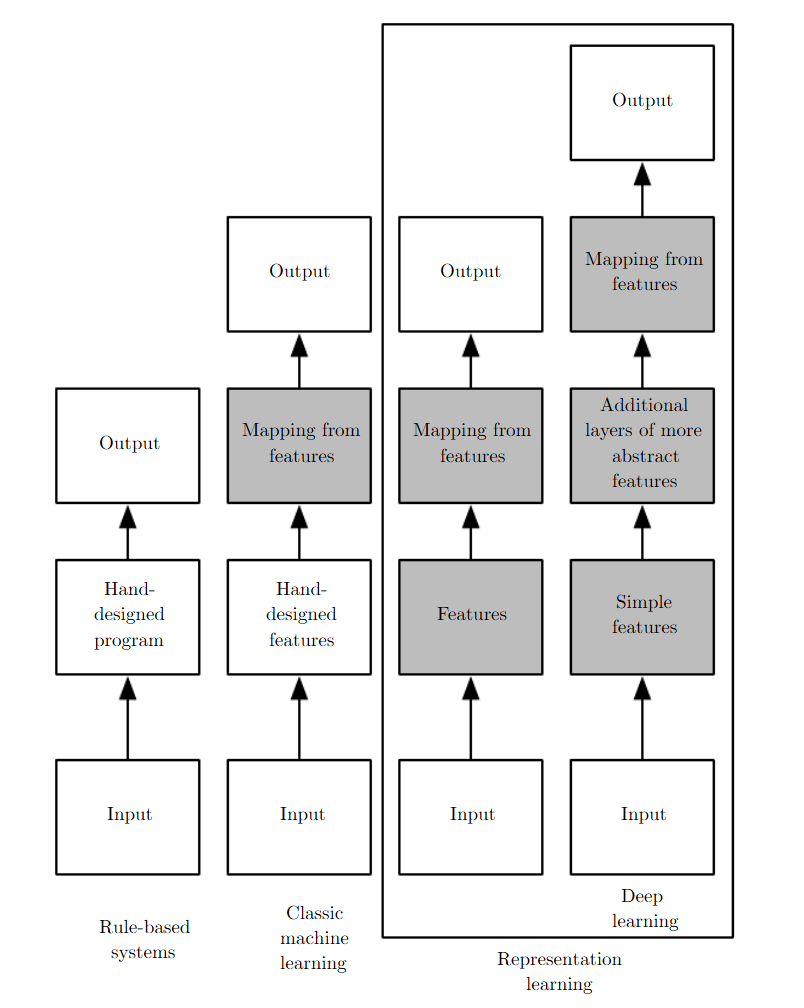
\includegraphics[width=0.75\linewidth]{Images/deepl-diff.png}
    \caption{Flowcharts showing the relation between different parts of an AI system}
\end{figure}
\defn{Knowledge Encoding}{
    Several artificial intelligence projects have sought to hard-code knowledge about
    the world in formal languages. A computer can reason automatically about statements
    in these formal languages using logical inference rules. This is known as the knowledge
    base approach to artificial intelligence. None of these projects has led to a major success.
    https://www.deeplearningbook.org/contents/intro.html
}

The diffculties faced by systems relying on hard-coded knowledge suggestthat AI systems 
need the ability to acquire their own knowledge, by extracting
patterns from raw data. This capability is known as machine learning.
The performance of these simple machine learning algorithms depends heavily
on the representation of the data they are given. (Example: Graph using Caresian vs Polar coordinates)


One solution to this problem is to use machine learning to discover not only
the mapping from representation to output but also the representation itself.
This approach is known as representation learning.
The quintessential example of a representation learning algorithm is the \textbf{autoencoder}.

\defn{Feature Design}{
    When designing features or algorithms for learning features, our goal is usually
    to separate the factors of variation that explain the observed data.

    The word "factors" simply to refer to separate sources of influence
}

When it is nearly as diffcult to obtain a representation as to solve theoriginal problem,
representation learning does not, at first glance, seem to help us.

\textbf{Deep learning} solves this central problem in representation learning by 
introducing representations that are expressed in terms of other, simpler representations.

\defn{Perspectives of Deep Learning}{
    The idea of learning the right representation for the data provides one perspective on deep learning.
    (Encodes factors of variation that explain the input)
    Another perspective on deep learning is that depth
    enables the computer to learn a multistep computer program.
}

\begin{figure}[H]
    \centering
    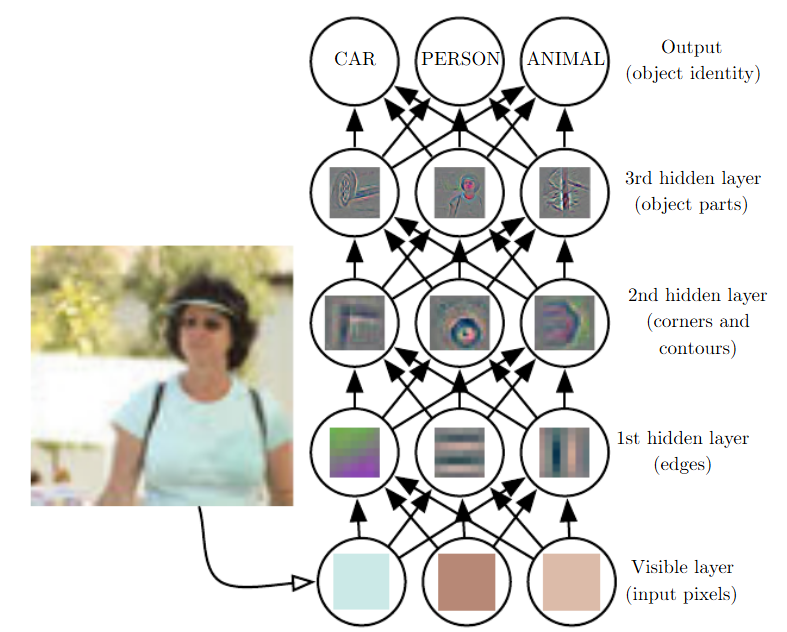
\includegraphics[width=0.75\linewidth]{Images/multistepalgorithm.png}
    \caption{An alorithm breaks a problem into feasable subproblems. It itself learns the data's representation.}
\end{figure}

\begin{figure}[H]
    \centering
    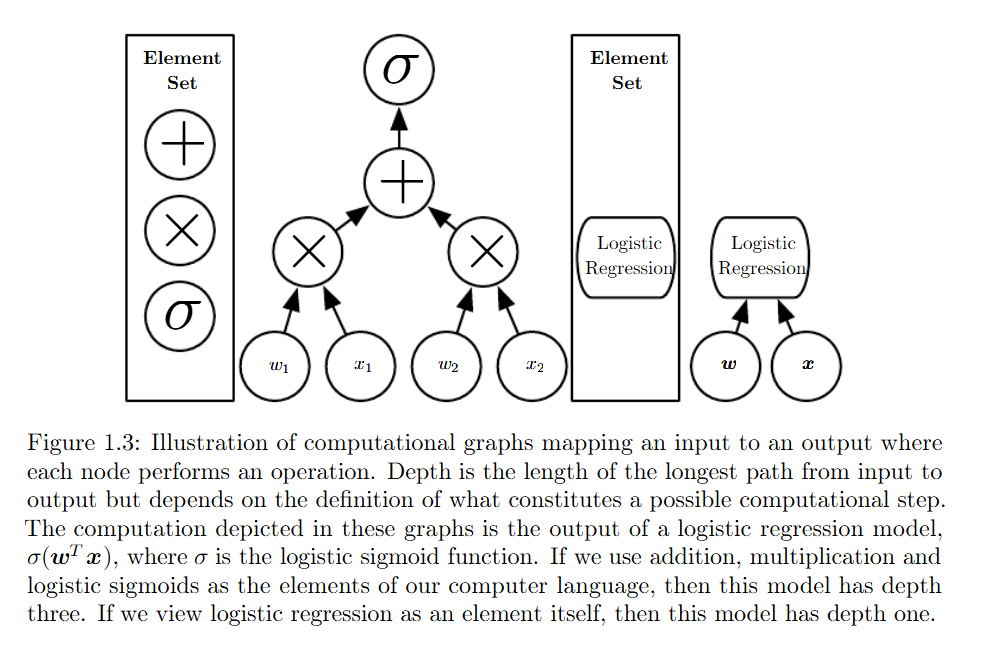
\includegraphics[width=0.75\linewidth]{Images/computational-depth.png}
\end{figure}

Deep learning can be safely regarded as thestudy of models that involve a greater amount of composition 
of either learned functions or learned concepts than traditional machine learning does.

\newpage
\section{Short Linear Algebra Recap}

\begin{figure}[H]
    \centering
    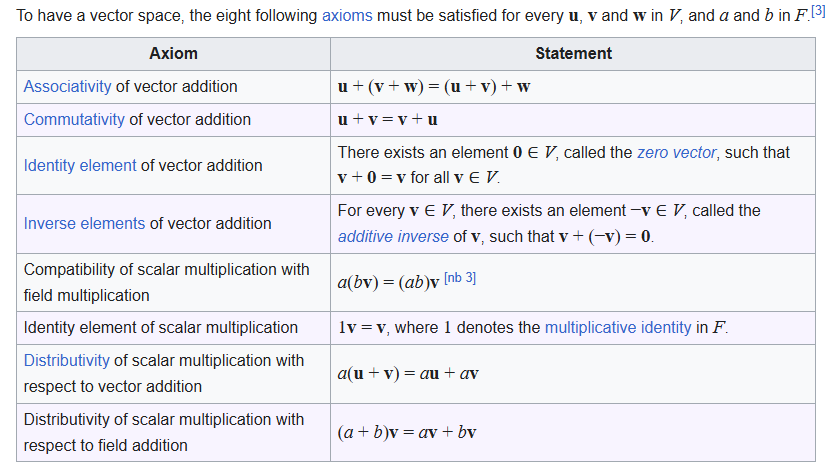
\includegraphics[width=0.75\linewidth]{Images/vector-space.png}
    \caption{Rules of a vector space}
\end{figure}

\begin{multicols}{2}
    Ein Skalar ist eine mathematische Größe,
    die allein durch die Angabe eines Zahlenwertes
    charakterisiert ist (in der Physik gegebenenfalls mit Einheit).
    \begin{equation}
        \text{Scalar} = s = 2
    \end{equation}

    \begin{equation}
        \text{Matrix} = \textbf{A} =
        \begin{bmatrix}
            1 & 2 & 3\\
            a & b & c
        \end{bmatrix} = \mathbb{R}^{2 \times 3}
    \end{equation}

    \begin{equation}
        \text{Vector} = \textbf{b} =
        \begin{bmatrix}
            1 \\
            a
        \end{bmatrix} = \mathbb{R}^2
    \end{equation}

    \begin{equation}
        \text{Tensor} = \mathbb{R}^{n_1 \times n_2 \times n_i}
    \end{equation}

    \begin{equation}
        \boldsymbol{I}_3 =
        \begin{bmatrix}
            1 & 0 & 0 \\
            0 & 1 & 0 \\
            0 & 0 & 1
        \end{bmatrix}
    \end{equation}
    The identity matrix can be thought of 
    as the matrix version of the number 1.
    \begin{equation}
        AA^{-1} = 1 = A^{-1}A
    \end{equation}
\end{multicols}

\defn{Diagonal Matrices}{
    \begin{equation}
        \begin{split}
            diag(\boldsymbol{v}) \Rightarrow D_{i,j} &= 0, \forall i \neq j \\
            diag(\boldsymbol{v}) \boldsymbol{x} &= \boldsymbol{v} \odot \boldsymbol{x} \\
            I_n &= diag(\boldsymbol{v})
        \end{split}
    \end{equation}

    Inverting diagonal matrices is 
    only possible, if all diagonal 
    elements are non-zero.
    \begin{equation}
        diag(v)^{-1} = diag([1/v_1, \cdots, 1/v_n]^T)
    \end{equation}

    \begin{itemize}
        \item Many generic machine learning 
        algorithms can be simplified by 
        restricting some matrices to be 
        diagonal matrices
    \end{itemize}
}

\defn{Symmetric Matrix}{
    Is a matrix that is equal to its transpose:
    \begin{equation}
        \boldsymbol{A} = \boldsymbol{A}^T
    \end{equation}
    \begin{equation*}
        \begin{bmatrix}
            1 & 1 & -1 \\
            1 & 2 & 0 \\
            -1 & 0 & 5
        \end{bmatrix}
    \end{equation*}
}

\defn{Orthonormal}{
    Ortho means that angle between the 
    vectors is a 90° angle and normal 
    means that the length of the vector is 
    one.
    In \(\mathbb{R}^n\), there are at most n such 
    vectors, which have a non-zero norm.
    \begin{equation}
        \begin{split}
            \boldsymbol{x}^T \boldsymbol{y} &= 0 \\
            ||\boldsymbol{x}||_2 &= 1
        \end{split}
    \end{equation}
}

\defn{Orthogonal Matrix}{
    An orthogonal matrix (should be 
    called an orthonormal matrix), is 
    a square matrix whose rows are 
    mutually orthonormal and whose 
    columns are mutually 
    orthonormal.

    \begin{equation}
        \boldsymbol{A}^T \boldsymbol{A} = \boldsymbol{A}^T = \boldsymbol{A}
    \end{equation}

    The the inverse is simply the transpose:
    \begin{equation}
        \boldsymbol{A}^{-1} = \boldsymbol{A}^T
    \end{equation}
}

\subsection{Products}

\defn{Dot Product}{
    \begin{equation}
        \boldsymbol{a} \cdot \boldsymbol{b} = \sum_{i} a_i b_i
    \end{equation}

    \begin{equation}
        \boldsymbol{x}^T \cdot \boldsymbol{y} = ||x||_2 ||y||_2 cos \theta
    \end{equation}
}

\defn{Matrix Product}{
    The matrix product C=AB is simply a matrix where \(C_{i,j}\) 
    is the dot product between row i of A and column j of B.
    \begin{equation}
        \begin{split}
            \boldsymbol{C} &= \boldsymbol{A} \boldsymbol{B} \neq \boldsymbol{B} \boldsymbol{A} \\
            C_{i,j} &= \sum_k A_{i,k} B_{k,j} \\
            A(B+C) &= AB + AC \\
            A(BC) &= (AB)C
        \end{split}
    \end{equation}
}

\defn{Hadamard Prod}{
    Is the element-wise product:
    \begin{equation}
        C = A \odot B
    \end{equation}
}

\begin{figure}[H]
    \centering
    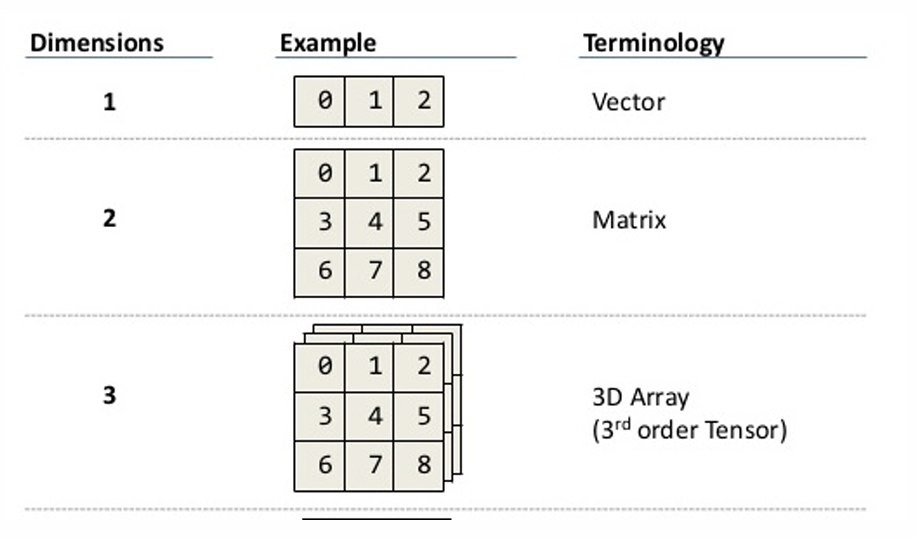
\includegraphics[width=0.75\linewidth]{Images/terminology-linalg.png}
    \caption{Linear Algebra Terminology}
\end{figure}

\defn{Multiplicative inverse}{
    Is a number which when multiplied by x yields the multiplicative identity, 1.
    In linear algebra we define an inverse matrix:
    \begin{equation}
        \boldsymbol{A}^{-1} \boldsymbol{A} = \boldsymbol{I}_n
    \end{equation}
}

\subsection{Solving Systems}
\defn{Lineare Gleichungssysteme}{
    Linear system of equations in its most compact form:
    \begin{equation}
        \boldsymbol{A} x = b \\
        A \in \mathbb{R}^{m \times n} \\
        b \in \mathbb{R}^m
    \end{equation}
    Oder auch anders geschrieben:
    \begin{equation}
        \begin{split}
            A_{1,1} x_1 + \cdots + A_{1,n} x_n &= b_1 \\
            \vdots & \\
            A_{m,1} x_1 + \cdots + A_{m,n} x_n &= b_m
        \end{split}
    \end{equation}

    Mit analytischer Lösung:
    \begin{equation}
        x = \boldsymbol{A}^{-1}b
    \end{equation}

   \begin{itemize}
    \item Mit Anzahl Lösungen:
    \begin{itemize}
        \item Keine, 1, Oder unendlich viele
    \end{itemize}
    \item  Note that using the inverse might 
            numerically not be the best approach.
 
    \item Requiring A to have the same or 
        more rows (n) than columns (m) 
        is a necessary condition for Ax=b 
        to have a unique solution.
        It is though not sufficient, since 
        the rows might be redundant.

    \item We need at least m 
        linearly independent column 
        vectors in A this will allow the 
        column space to cover \(\mathbb{R}^m\)

    \item If we want Ax=b to have at most one 
    solution, we require 
    that there are at most m columns. 
    Otherwise, there is more than one 
    way of parameterizing each solution
    Hence for \(A^{-1}\) to exist, we require 
    m=n, where all the columns are linearly independent
   \end{itemize}
}

\defn{Span}{
    A matrix contains column vectors 
    \(A_{:,i}\) , hence Ax can be interpreted 
    as a linear combination of these vectors.
    It can be imagined as a vector 
    pointing from the origin into space 
    and hence Ax is the weighted 
    concatenation of these vectors.

    \begin{equation}
        \boldsymbol{Ax} = \sum_i x_i \boldsymbol{A}_{:,i}
    \end{equation}

    The span of a set of vectors is now 
    defined as the set of all points 
    obtainable by linear combinations of 
    these vectors.
}

\begin{figure}[H]
    \centering
    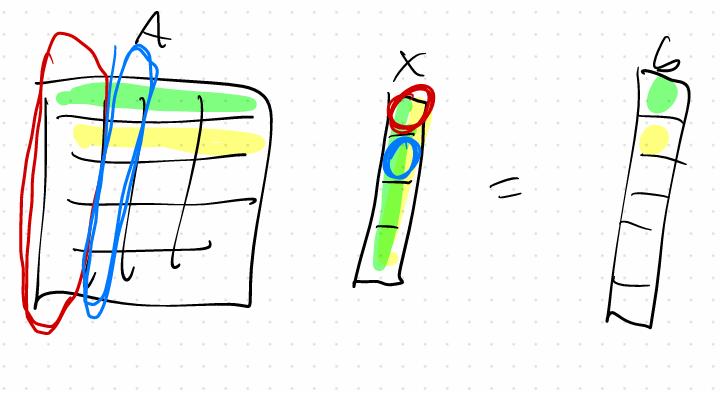
\includegraphics[width=0.75\linewidth]{Images/span.png}
    \caption{Span}
\end{figure}

\defn{Column Space of A}{
    Ax=b has only a solution, if b is in the span of the columns of A.
    This is called the column space of A or the range of A. Since this has to hold for each 
    vector b, and b is of dimensions 
    mx1, this implies that A 
    (dimensions mxn) must have at 
    least m columns, i.e., n>=m.
}

\defn{Rank}{
    The dimension of the column space is called the rank of the matrix.
}

\begin{figure}[H]
    \centering
    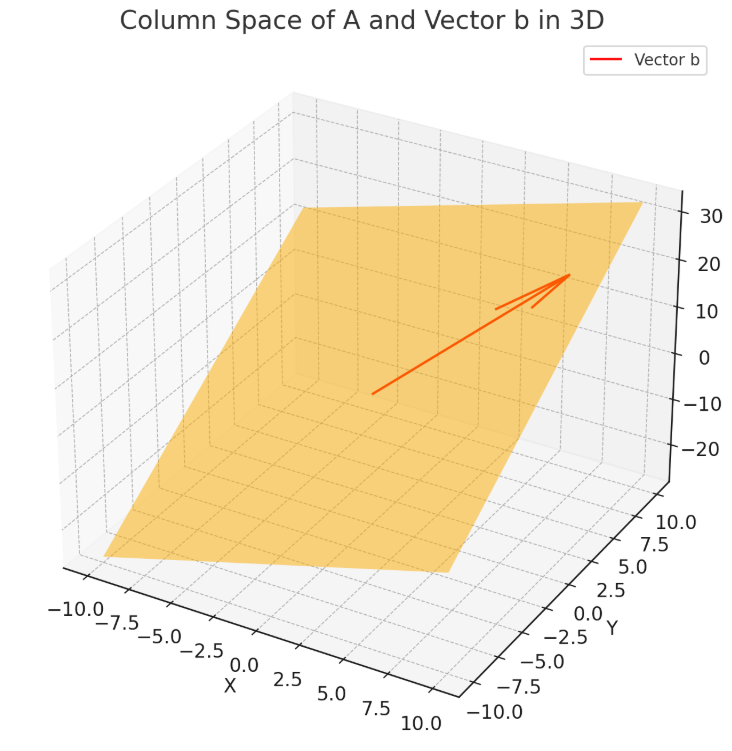
\includegraphics[width=0.5\linewidth]{Images/col-space-1.png}
    \caption{The 3D visualization of the column space of A,
    with the plane showing the span of the columns of A,
    and the red vector representing b. 
    If b b lies in this plane, it is in the column space, meaning a solution exists.an}
\end{figure}
\begin{figure}[H]
    \centering
    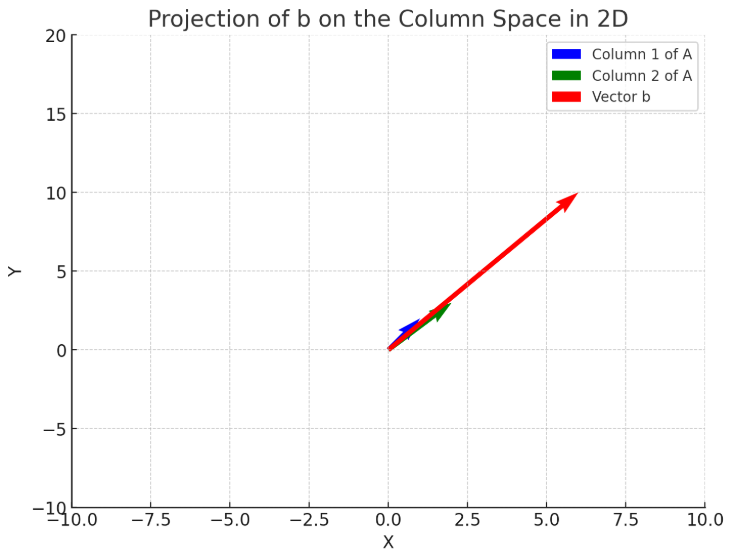
\includegraphics[width=0.5\linewidth]{Images/col-space-2.png}
    \caption{A 2D projection of the column space, showing how vector 
    b can be decomposed in terms of the two columns of A.
    If b lies within the span of these columns (the plane), a solution can be found.}
\end{figure}

\defn{Linear Independence}{
    Vector spaces, a set of vectors is said to be linearly independent if there exists
    no nontrivial linear combination of the vectors that equals the zero vector.
    If such a linear combination exists, then the vectors are said to be linearly dependent.
    \begin{equation}
        a_1 v_1 + a_2 v_2 + \cdots + a_k v_k = 0
    \end{equation}
    With at least one of the scalars is nonzero.

    Or with other words:
    A set of vectors is linearly 
    independent, if no vector in the set is 
    a linear combination of the other 
    vectors
}

\subsection{Norms}
\defn{Norm}{
    A norm is a way to measure the length of a vector.

    \begin{equation}
        \begin{split}
            f(x) &= 0 \Rightarrow x = 0 \\
            f(x+y) &\leq f(x) + f(y) \text{ triangle inequality} \\
            \forall \alpha \in \mathbb{R}, f(\alpha x) &= |\alpha| f(x)
        \end{split}
    \end{equation}
}

\defn{\(L^p\) Norm}{
    The euclidian norm is the \(L^p\) norm with p=2.
    \begin{equation}
        ||x||_p = (\sum_i |x_i|^p)^{\frac{1}{p}} \text{ for } p \in \mathbb{R},p \geq 1
    \end{equation}

    \begin{equation}
        ||x||_1 = \sum_{i} |x_i|
    \end{equation}

    \begin{equation}
        ||x||^2 = x^T x
    \end{equation}

    \begin{itemize}
        \item Close to zero, the squared norm increases very slowly
    \end{itemize}
}

\defn{Max Norm}{
    \(L^{\infty}\) norm which simplifies:
    \begin{equation}
        \begin{split}
            ||x||_{\infty} = \underset{i}{max} |x_i|
        \end{split}
    \end{equation}
}

\defn{Frobenius Norm}{
    Measures the size of a matrix, in a similar manner as the \(L^2\).
    \begin{equation}
        ||\boldsymbol{A}||_F = \sqrt{\sum_{i,j} A^2_{i,j}}
    \end{equation}
    \begin{equation}
        ||\boldsymbol{A}||_F = \sqrt{Tr(\boldsymbol{A}\boldsymbol{A}^T)}
    \end{equation}
}

\defn{Broadcasting}{
    In Deep Learning, it is common to 
    add scalars to matrices, which 
    means, that the scalar is added at 
    every entry of the matrix.
    \begin{equation}
        D = a \boldsymbol{B} + c
    \end{equation}

    It is further common to add 
    vectors to matrices, which means 
    that the vector is added to every 
    column of the matrix
    \begin{equation}
        \boldsymbol{C} = \boldsymbol{A} + \boldsymbol{b} \text{ where } C_{i,j} = A_{i,j} + b_j
    \end{equation}
}

\subsection{Matrix Decompositions}

\defn{Eigenvector / Eigenvalue}{
    a non-zero vector \textbf{v} that satisfies the eigen-equation is called an 
    eigenvector of \textbf{A} and the scalar \(\lambda\) 
    the corresponding eigenvalue:
    \begin{equation}
        \boldsymbol{Av} = \lambda \boldsymbol{v}
    \end{equation}

    This equation implies that any vector 
    \textbf{v} that is transformed by matrix \textbf{A} into 
    itself (except a scaling factor \(\lambda\)) is an 
    eigenvector of A. Hence the word 
    "Eigen", since the vector stays itself.

    To find eigenvalues of B use:
    \begin{equation}
        \begin{split}
            det(\boldsymbol(B) - \lambda \boldsymbol{I}) = 0 \\
            \Rightarrow = \lambda_1, \cdots, \lambda_n
        \end{split}
    \end{equation}
    Für eigenvektoren:
    \begin{equation}
        (\boldsymbol{B} - \lambda_i \boldsymbol{I})v_i = \boldsymbol{0}
    \end{equation}
}

\defn{Eigendecomposition}{
    Decomposing a matrix into a set of eigenvectors and eigenvalues.
    \textbf{Focus on real symmetric matrices.}

    Assume that \textbf{A} has n linearly 
    independent eigenvectors and 
    corresponding eigenvalues
    Now we can concatenate these 
    eigenvectors to form a matrix \textbf{V} 
    and concatenate the 
    corresponding eigenvalues to 
    form the vector \(\lambda\):
    \begin{equation}
        \begin{split}
            \boldsymbol{V} &= [\boldsymbol{v}^{(1),} \cdots, \boldsymbol{v}^{(n)}] \\
            \boldsymbol{A} &= \boldsymbol{V} diag(\boldsymbol{\lambda}) \boldsymbol{V}^{-1}
        \end{split}
    \end{equation}

    \textbf{Every real and symmetric matrix has a eigendecomposition!}
    The eigenvectors are guaranteed to be orthogonal.
    \begin{equation}
        \boldsymbol{A} = \boldsymbol{Q\Lambda} \boldsymbol{Q}^T
    \end{equation}
    Because \textbf{Q} is orthogonal we can write \(\boldsymbol{Q}^T\) instead of \(\boldsymbol{Q}^{-1}\)
}

Solving the system of equations \( Ax = b \) using eigendecomposition:

1. If \( A \) is symmetric, we can decompose it as:
   \[
   A = Q \Lambda Q^T
   \]
   where \( Q \) is orthogonal (\( Q^T = Q^{-1} \)) and \( \Lambda \) is diagonal.

2. Substitute into the system:
   \[
   Q \Lambda Q^T x = b
   \]

3. Multiply both sides by \( Q^T \):
   \[
   \Lambda Q^T x = Q^T b
   \]

4. Define \( y = Q^T x \), so that:
   \[
   \Lambda y = Q^T b
   \]

5. Since \( \Lambda \) is diagonal, solve for \( y \) component-wise:
   \[
   y_i = \frac{(Q^T b)_i}{\lambda_i}, \quad \text{for } \lambda_i \neq 0
   \]

6. Transform back to \( x \):
   \[
   x = Q y
   \]

Thus, we solve the system efficiently by diagonalizing \( A \), transforming \( b \), solving simple equations, and transforming back.

\begin{figure}[H]
    \centering
    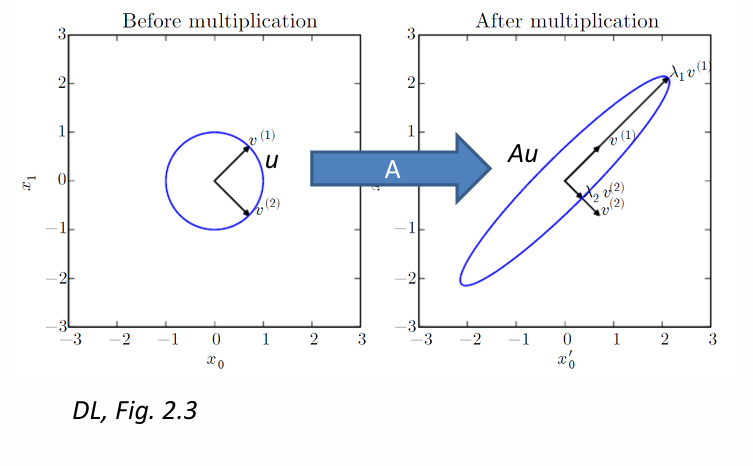
\includegraphics[width=0.75\linewidth]{Images/eigendecomp.png}
    \caption{Eigendecomposition, Blue Circle = All possible points reached using unit vectors,
    We then apply matrix \textbf{A} to each point. Eigenvectors are just scaled by the transformation by a eigenvalue}
\end{figure}

\defn{Eigendecomposition in Optimization}{
    For:
    \begin{equation}
        f(\boldsymbol{x}) = \boldsymbol{x}^T \boldsymbol{Ax} \text{ subject to } ||\boldsymbol{x}||_2 = 1
    \end{equation}
    If x is a unit eigenvector of A, then:
    \begin{equation}
        \begin{split}
            \boldsymbol{Ax} &= \lambda \boldsymbol{x} \\
            \boldsymbol{x}^T \boldsymbol{Ax} &= \boldsymbol{x}^T \lambda \boldsymbol{x} \\
            &= \lambda
        \end{split}
    \end{equation}
    \begin{itemize}
        \item The maximum of this function is now 
        found for the vector x corresponding 
        to the eigenvector belonging to the 
        maximum eigenvalue.
        \item Similarly, the minimum of the 
        function f(x) is the eigenvector 
        belonging to the minimum 
        eigenvalue.
    \end{itemize}
}

\defn{Singular Value Decomposition (SVD)}{
    Is a more general way of factoring a matrix into singular vectors and values.
    Every real matrix has an SVD.
    \begin{equation}
        \boldsymbol{A} = \boldsymbol{UD} \boldsymbol{V}^T
    \end{equation}
    \begin{description}
        \item[A] mxn Matrix
        \item[U] An orthogonal mxm matrix. Cols are called left-singular vectors, these are eigenvectors of \(AA^T\).
        Note that \(u^{(1)}\) is the eigenvector to the largest eigenvalue.
        \item[D] Diagonal mxn matrix. The diagonal elements are called singular values. Non-zero sv are square roots of eigenvalues of \(AA^T\).
        Note that: \(\lambda_1 > \lambda_2\)
        \item[V] Orthogonal nxn matrix. Cols are called right-singular vectors and are eigenvectors of \(A^T A\)   
        Note that \(v^{(1)}\)is the eigenvector to the larger eigenvalue \(\lambda_1\).
    \end{description}
}

\subsection{Pseudoinverse}
The inverse of a matrix is undefined if its not square.
This means that the inverse is of little use in deep learning.
What we really want is in a underdefined or overdefined problem to find the best fitting solution.
\defn{Moore-Penrose Pseudoinverse}{
    The Moore-Penrose 
    pseudoinverse allows for a 
    reasonable solution in both cases (under or overdefined)
    and is defined as a limit.
    \begin{equation}
        \begin{split}
            \boldsymbol{A}^+ &= \lim_{a\searrow 0}( \boldsymbol{A}^T  \boldsymbol{A} + \alpha  \boldsymbol{I})^{-1}  \boldsymbol{A}^T \\
            \boldsymbol{A}^+ &=  \boldsymbol{V}  \boldsymbol{D}^+  \boldsymbol{U}^T
        \end{split}
    \end{equation}

    Note the similarity to the SVD, 
    basically the pseudoinverse is the 
    transpose of A=UD\(V^T\), which 
    would result in \(A^T=VD^TU^T\)
    \textbf{The transpose is simply the 
    inverse for orthogonal matrixes 
    (U and V) but not for D}. With:
    \begin{equation}
        D^+_{i,i} = 1/D_{i,i} 
    \end{equation}
    the diagonal elements are inverted
    and then the matrix is transposed!

    \begin{equation}
        \boldsymbol{A}^+ \boldsymbol{A} = \boldsymbol{I}
    \end{equation}

    \begin{itemize}
        \item When there are more unknowns 
        (columns n) than equations (rows 
        m), then the pseudoinverse 
        returns the shortest vector 
        \(x=A^+y\), among all possible 
        solutions.
        \begin{equation*}
            \boldsymbol{x} = \boldsymbol{A}^+\boldsymbol{y} \text{ with minimal } ||\boldsymbol{x}||_2
        \end{equation*}
        \item When there are more equations 
        (rows m) than unknowns 
        (columns n), then the 
        pseudoinverse returns the vector 
        x such that Ax is as close as 
        possible to the vector y
        \begin{itemize}
            \item RSS/MSE optimal solution
        \end{itemize}
        \begin{equation*}
            \begin{split}
                \boldsymbol{Ax} &= \boldsymbol{y} \\
                \Rightarrow &min(||\boldsymbol{Ax} - \boldsymbol{y}||_2)
            \end{split}
        \end{equation*}
    \end{itemize}
}

\exm{Pseudoinverse}{
    We want to solve \(Ax=b\) where    
    \begin{equation*}
        \begin{split}
            A &= \begin{bmatrix}
                1 & 2 \\
                1 & 4 \\
                1 & 6
            \end{bmatrix}, \\
            b &= \begin{bmatrix}
                1.8 \\
                3.3 \\
                4.1
            \end{bmatrix}
        \end{split}
    \end{equation*}
    First calculate D. Recapulate that from SVD the following is given:
    \begin{equation*}
        A = UDV^T
    \end{equation*}
    Where in D the diagonal elements are the square roots of eigenvalues of \(AA^T\)
    \begin{equation*}
        \begin{split}
            B &= A^TA \\
            \Rightarrow \\
            det(B-\lambda I) &= 0 \\
            (3-\lambda)(56-\lambda)-(12*12) &= 0 \\
            \lambda_1 &= 58.59, \lambda_2 = 0.409
        \end{split}
    \end{equation*}
    Now we can define D:
    \begin{equation*}
        \begin{split}
            D &= \begin{bmatrix}
                \sqrt{\lambda_1} & 0 \\
                0 & \sqrt{\lambda_2} \\
                0 & 0
            \end{bmatrix} \\
            D &= \begin{bmatrix}
                7.6544 & 0 \\
                0 & 0.6400 \\
                0 & 0
            \end{bmatrix}
        \end{split}
    \end{equation*}
    Now determine matrix V where \(v^{(i)}\) are eigenvectors of B.
    \begin{equation*}
        \begin{split}
            (\boldsymbol{B} - \lambda_i \boldsymbol{I})v_i &= \boldsymbol{0} \\
            \Rightarrow \text{for } \lambda_1 \\
            (\begin{bmatrix}
                3 & 12\\
                12 & 56
            \end{bmatrix} - 58.59 I)v_1 &= \boldsymbol{0} \\
            \begin{bmatrix}
                -55.59x & 12y\\
                12x & -2.59y
            \end{bmatrix}&= 0 
        \end{split}
    \end{equation*}

    \begin{equation*}
        \begin{split}
            \text{Solve linear equation} \\
            v_1 = (0.216,1)^T \\
            \text{Now normalize} \\
            ||v_1||= (0.211,0.978)^T \\
            \text{Repeat for } v_2 \\
            \Rightarrow \\
            V = \begin{bmatrix}
                -0.2110 & -0.9775\\
                -0.9775 & 0.2110
            \end{bmatrix}
        \end{split}
    \end{equation*}

    Now determine \(U =(u^{(1)}, u^{(2)}, u^{(3)})\) using \(C=AA^T\)
    \begin{equation*}
        U = \begin{bmatrix}
            -0.2830 & -0.8679 & 0.4082\\
            -0.5384 & -0.2085 & -0.8165\\
            -0.7938 & 0.4508 & 0.4082
        \end{bmatrix}
    \end{equation*}

    Now check if U and V are orthogonal:
    \begin{equation*}
        \begin{split}
            UU^T = I \\
            VV^T = I
        \end{split}
    \end{equation*}

    Check if SVD matches:
    \begin{eqnarray*}
        A = UDV^T
    \end{eqnarray*}

    Now for the Moore-Penrose calculate \(D^+\):
    \begin{equation*}
        \begin{split}
            D_{i,i}^+ = 1/D_{i,i} \\
            D^+ = \begin{bmatrix}
                \frac{1}{\lambda_1} & 0\\
                0 & \frac{1}{\lambda_2}\\
                0 & 0
            \end{bmatrix}^T \\
            = \begin{bmatrix}
                0.1307 & 0 & 0 \\
                0 & 1.5625 & 0
            \end{bmatrix}
        \end{split}
    \end{equation*}

    Now asselbe the Moore-Penrose pseudo inverse:
    \begin{equation*}
        A^+ = VD^+ U^T = = \begin{bmatrix}
           4/3 & 1/3 & -2/3 \\
            -1/4 & 0 & 1/4
        \end{bmatrix}
    \end{equation*}

    Now since there are more equations than 
    unknowns the optimal RSS/MSE solution can be calculated:
    \begin{equation*}
        \begin{split}
            Ax = b | A^+\\
            x = A^+ b \\
            \begin{bmatrix}
                4/3 & 1/3 & -2/3 \\
                 -1/4 & 0 & 1/4
             \end{bmatrix} \begin{bmatrix}
                1.8 \\
                3.3 \\
                4.1
            \end{bmatrix} = x \\
            x = \begin{bmatrix}
                0.7667 \\
                0.5750
            \end{bmatrix}
        \end{split}
    \end{equation*}
}

\subsection{Trace and Determinant}

\defn{Trace}{
    \begin{equation}
        Tr(\boldsymbol{A}) = \sum_{i} A_{i,i}
    \end{equation}
    Used to replace a sum over some squared errors.
    \begin{equation*}
        ||\boldsymbol{A}||_F = \sqrt{Tr(\boldsymbol{A}\boldsymbol{A}^T)}
    \end{equation*}

    \begin{equation}
        \begin{split}
            Tr(\boldsymbol{A}^T) &= Tr(\boldsymbol{A}) \\
            Tr(\boldsymbol{AB}) &= Tr(\boldsymbol{BA}) \\
            Tr(\boldsymbol{ABC}) &= Tr(\boldsymbol{CAB}) = Tr(\boldsymbol{BCA}) \\
            Tr(A) &= \sum_{i} \lambda_i
        \end{split}
    \end{equation}
    The trace is the sum of all eigenvalues.
}

\defn{Determinant}{
    \begin{equation}
        det(\boldsymbol{A}) = \prod_{i} \lambda_i
    \end{equation}
}


\begin{figure}[H]
    \centering
    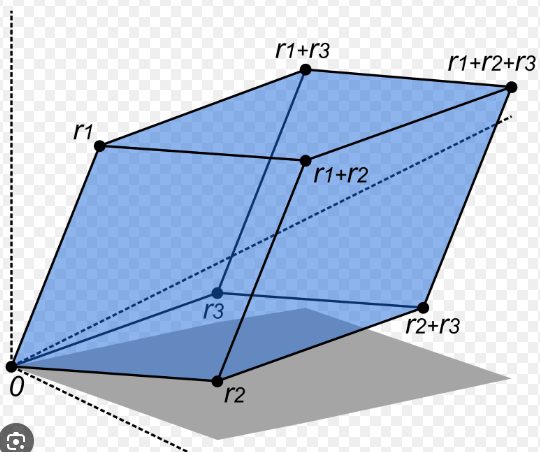
\includegraphics[width=0.5\linewidth]{Images/determinant.png}
    \caption{In 3D space the determinant shows the change in volume after the transformation. (in 2D the area)}
\end{figure}

\section{Ergänzungen DMI}
\begin{figure}[H]
    \centering
    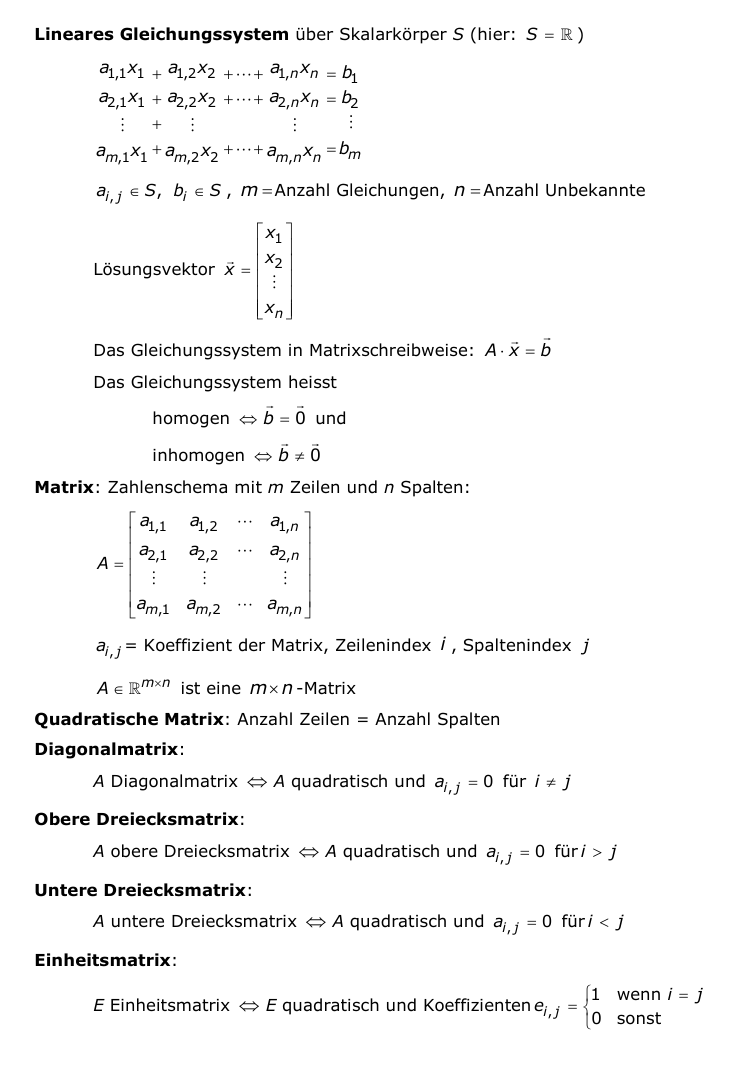
\includegraphics[width=0.75\linewidth]{Images/dmi_1.png}
    \caption{LinAlg Zusammenfassung 1}
\end{figure}

\begin{figure}[H]
    \centering
    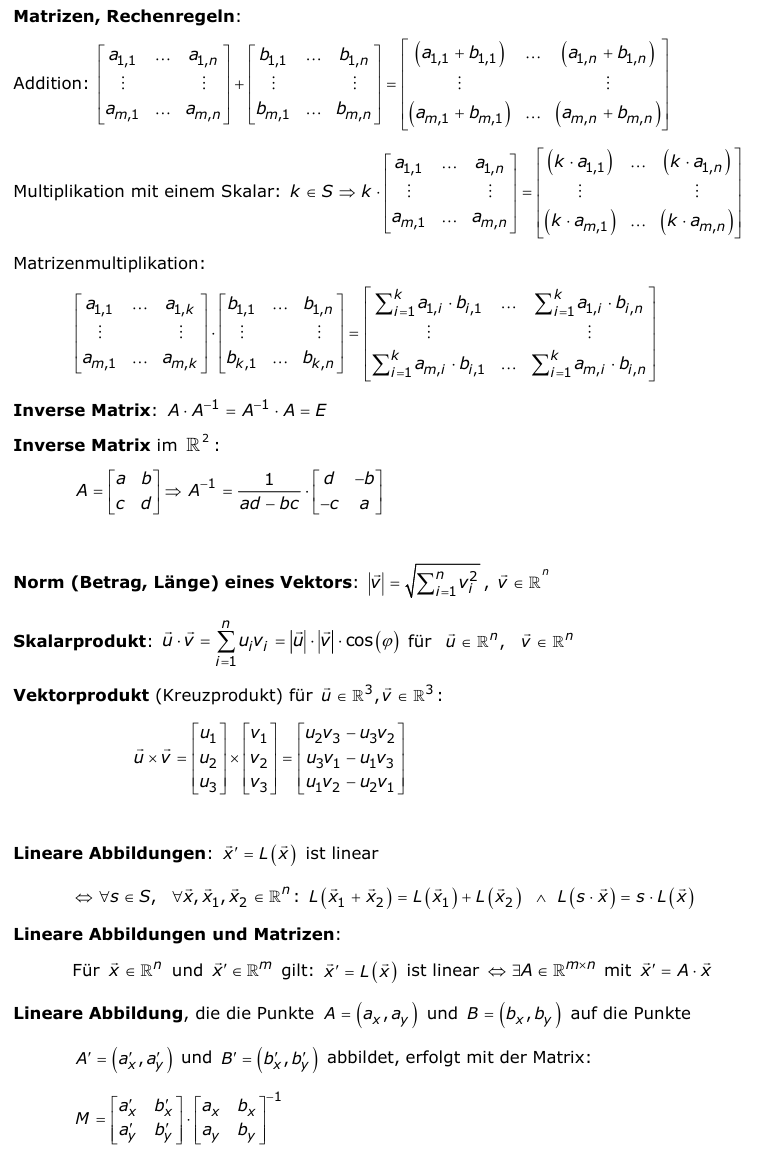
\includegraphics[width=0.75\linewidth]{Images/dmi_2.png}
    \caption{LinAlg Zusammenfassung 2}
\end{figure}

\begin{figure}[H]
    \centering
    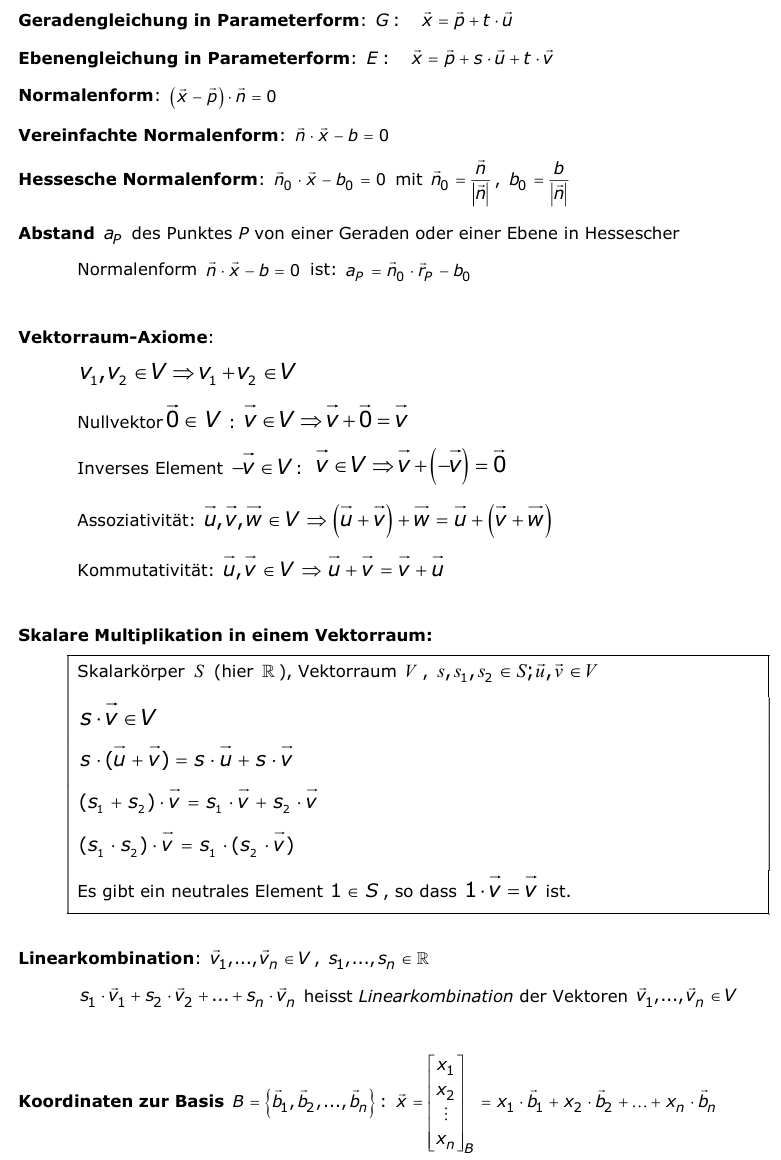
\includegraphics[width=0.75\linewidth]{Images/dmi_3.png}
    \caption{LinAlg Zusammenfassung 3}
\end{figure}

\begin{figure}[H]
    \centering
    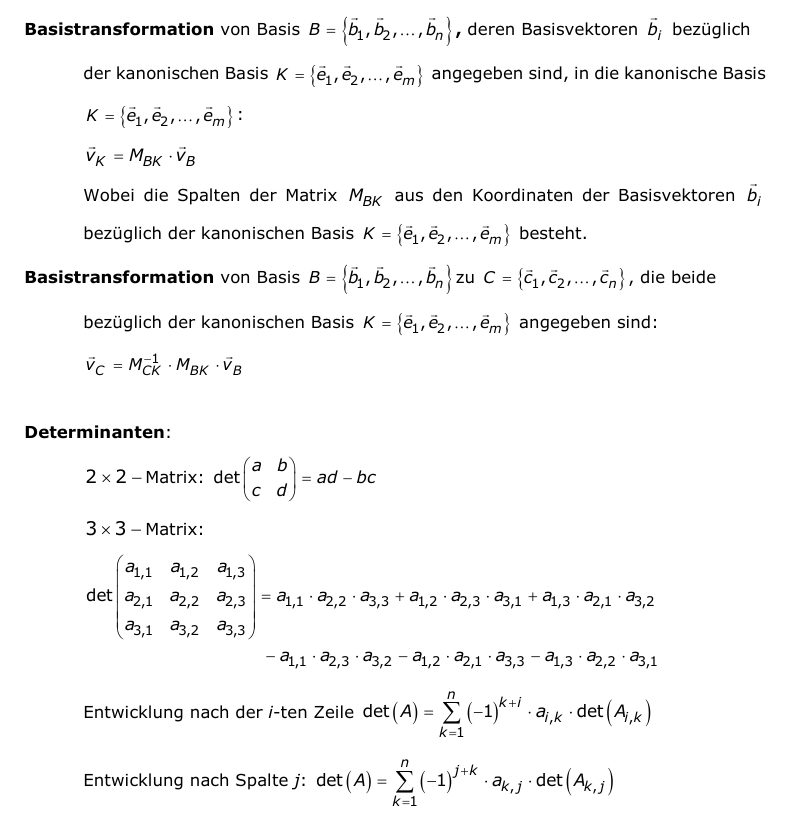
\includegraphics[width=0.75\linewidth]{Images/dmi_4.png}
    \caption{LinAlg Zusammenfassung 4}
\end{figure}

\section{Ergänzungen Wahrscheinlichkeiten}

\subsection{Sources of uncertainty}
\begin{itemize}
    \item Inherent stochasticity in the system being modeled
    \item Incomplete observability
    \item Incomplete modeling
\end{itemize}

\subsection{Recap}

\defn{Discrete Random Variables - Probability Mass Functions (PMF)}{
    \begin{equation}
        \begin{split}
            X &\sim P(X) \\
            \text{Domain of } P(X) &= \text{ all possible states} \\
            0 &\leq P(x) \leq 1 \\
            \sum P(X) &= 1
        \end{split}
    \end{equation}
    Note that probability 0 is not impossible as 
    stated on the right but improbable vice versa for 1.
}

\defn{Continues Random Variables - Probability Density Functions}{
    In englisch we explicitly differentiate with using the term "density"
    or even better "likelyhood".
    \begin{equation}
        \begin{split}
            X &\sim p(X) \\
            \text{Domain of } P(X) &= \text{ all possible values} \\
            0 &\leq P(x) \\
            \int P(X) &= 1 \\
            P(a \leq x \leq b) &= \int_{a}^{b} p(x) dx
        \end{split}
    \end{equation}
}

\defn{Uniform PDF}{
    \begin{equation}
        X \sim U(a,b) = \frac{1}{b-a}
    \end{equation}
}

\defn{Marginalization}{
    Simply sum (integrate) over all 
    variables one is not interested in. These distributions are then called 
    marginal probability distributions, 
    but they are just pmf/pdf of the particular rv.
    \begin{equation}
        \begin{split}
            \forall x \in X, P(X=x) = \sum_{y} P(X=x, Y=y) \\
            p(x) = \int p(x,y) dy
        \end{split} 
    \end{equation}
}

\defn{Conditional Probability}{
    \begin{equation}
        P(Y=y | X=x)= \frac{P(Y=y, X=x)}{P(X=x)}
    \end{equation}
    Or use Bayes!
    \begin{equation}
        \begin{split}
            P(X|Y) &= \frac{P(X)}{P(Y)} P(Y|X) \\
            P(Y) &= \sum_{X} P(Y|X) P(X)
        \end{split}
    \end{equation}
    Note:
    \begin{equation*}
        P(x|y)P(y)=P(x,y)=P(y,x)=P(y|x)P(x)
    \end{equation*}
}

\begin{figure}[H]
    \centering
    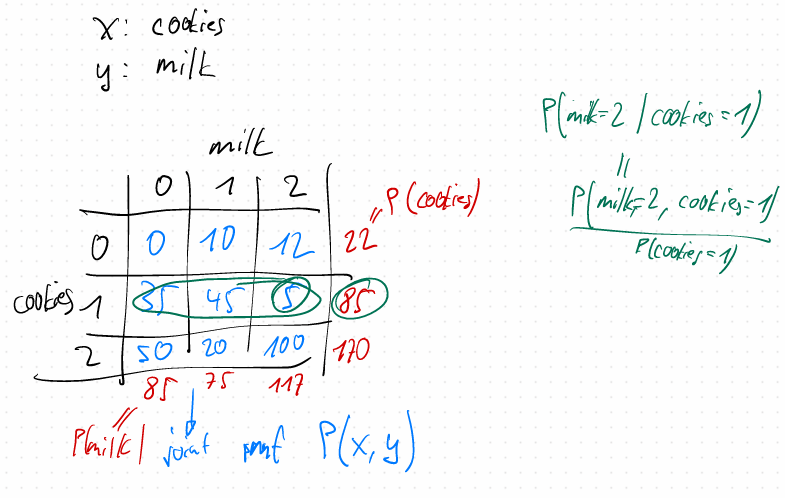
\includegraphics[width=0.5\linewidth]{Images/jointprob.png}
    \caption{Marginalization}
\end{figure}

\defn{Chain Rule of Conditional Probabilities}{
    \begin{equation}
        P(x^{(1)},\cdots,x^{(n)}) = P(x^{(1)}) \prod_{i=2}^{n} P(x^{(i)} | x^{(1)},\cdots,x^{(i-1)})
    \end{equation}
    This follows from:
    \begin{equation*}
        \begin{split}
            P(Y=y | X=x) &= \frac{P(Y=y, X=x)}{P(X=x)} \\
            \Rightarrow \\
            P(a,b,c) &= P(a|b,c)P(b,c) \\
            P(b,c) &= P(b|c)P(c) \\
            P(a,b,c) &= P(a|b,c)P(b|c)P(c)
        \end{split}
    \end{equation*}
}

\defn{Statistical Independence}{
    \begin{equation}
        \begin{split}
            \forall x \in X, y \in Y, p(X=x,Y=y) = p(X=x)p(Y=y)\\
            = x \perp y
        \end{split}
    \end{equation}
    This also applies for conditionals:
    \begin{equation}
        \begin{split}
            x \perp y | z \\
            = p(X=x | Z=z) p(Y=y | Z=z)
        \end{split}
    \end{equation}
}

\defn{Different Notation for Excpectation}{
    \begin{equation}
        \begin{split}
            \mathop{\mathbb{E}}_{x \sim P}[f(x)] &= \sum_{x} P(x)f(x) \\
            \mathop{\mathbb{E}}_{x \sim p}[f(x)] &= \int p(x) f(x) dx
        \end{split}
    \end{equation}
    With simplified notation:
    \begin{equation}
        \begin{split}
            \mathop{\mathbb{E}}_x[f(x)]\\
            \mathop{\mathbb{E}}[f(x)]
        \end{split}
    \end{equation}
    \begin{itemize}
        \item Expectation is a linear operator
    \end{itemize}
}

\defn{Different Notation for Variance}{
    The variance measures the expected 
    squared distance of f(x) to its 
    expected value E[f(x)].
    \begin{equation}
        Var(f(x)) = \mathop{\mathbb{E}}[(f(x)-\mathop{\mathbb{E}}[f(x)])^2]
    \end{equation}
}

\defn{Different Notation for Covariance}{
    Gives some insights 
    of how much two rvs are linearly 
    related to each other and also 
    the scale of these rvs.

    \begin{equation}
        Cov(f(x),g(x)) = \mathop{\mathbb{E}}[(f(x)- \mathop{\mathbb{E}}[f(x)]) (g(y)-\mathop{\mathbb{E}}[g(y)])]
    \end{equation}

    The correlation is the covariance 
    divided by the standard deviations of 
    f(x) and f(y) and can only be in the 
    range of -1 to +1:
    \begin{equation}
        p_{X,Y} = corr(X,Y) = \frac{cov(X,Y)}{\sigma_X \sigma_Y}
    \end{equation}

    Independent rvs have a 
    covariance of 0 but a covariance 
    of 0 does not necessarily mean, 
    that the rvs are independent
}

\defn{Covariance Matric}{
    Of a random vector \(\boldsymbol{x} \in R^n\) is a nxn matrix, such that:
    \begin{equation}
        Cov(x)_{i,j} = Cov(x_i, x_j)
    \end{equation}
    The diagonal elements give the variance:
    \begin{equation}
        Cov(x_i, x_i) = Var(x_i)
    \end{equation}
}

\begin{figure}[H]
    \centering
    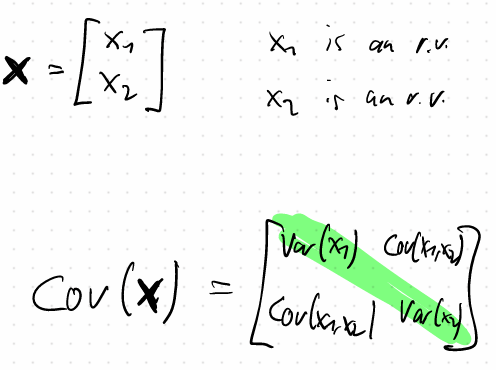
\includegraphics[width=0.5\linewidth]{Images/covmatrix.png}
    \caption{Covariance Matrix}
\end{figure}

\section{Further Distributions}
\defn{Bernoulli}{
    \begin{equation}
        \begin{split}
            P(x=1) = \phi \\
            P(x=0) = 1- \phi \\
            \mathop{\mathbb{E}}[x] = \phi \\
            Var(x) = \phi(1-\phi)
        \end{split}
    \end{equation}
}

\begin{figure}[H]
    \centering
    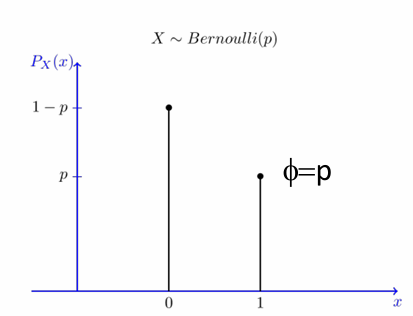
\includegraphics[width=0.5\linewidth]{Images/bernoulli-d.png}
    \caption{Bernoulli Distribution}
\end{figure}

\defn{Multinoulli}{
    Distribution over a discrete variable with k states \(p \in [0,1]^{k-1}\).
    \textbf{p} is a vector with k-1 elements, where each entry \(p_i\) is the probability of state i.

    The final states probability 
    \(p_k\) is given by:
    \begin{equation}
        p_k = 1-\boldsymbol{1}^T \boldsymbol{p}
    \end{equation}

    Used to describe probabilities over a finite number of classes.
}

\defn{Gaussian}{
    \begin{equation}
        N(x; \mu, \sigma^2) = \sqrt{\frac{1}{2 \pi \sigma^2}} exp(-\frac{1}{2\sigma^2} (x-\mu)^2)
    \end{equation}
    Alternative parameterization, where \(\beta\) is called the precision:
    \begin{equation}
        N(x; \mu, \beta^{-1}) = \sqrt{\frac{\beta}{2 \pi}} exp(-\frac{1}{2}\beta (x-\mu)^2)
    \end{equation}
    \(\beta\) is simply \(\frac{1}{\sigma^2}\)


    \begin{itemize}
        \item central limit theorem, which 
        states that the sum of many 
        independent rvs approaches a 
        Gaussian distribution
        \item For a given variance, the Gaussian 
        distribution has the largest 
        uncertainty (differential entropy) 
    \end{itemize}
    \begin{equation*}
        h(X) = - \int_{X} f(x) log f(x) dx
    \end{equation*}
    An in multiple dimensions:
    \begin{equation}
        N(x; \mu, \Sigma) = \sqrt{\frac{1}{(2 \pi)^n det(\Sigma)}} exp(-\frac{1}{2}(x-\mu)^T \Sigma^{-1} (x-\mu)^2)
    \end{equation}
    \begin{equation}
        N(x; \mu, \beta^{-1}) = \sqrt{\frac{det(\beta)}{(2 \pi)^n }} exp(-\frac{1}{2}(x-\mu)^T \beta (x-\mu)^2)
    \end{equation}
    \begin{itemize}
        \item For simplicity, the covariance matrix 
        is often assumed to be a diagonal 
        matrix, hence all dimensions of x are 
        uncorrelated
        \item An even simpler model is the 
        isotropic Gaussian distribution since 
        the covariance matrix is simply a 
        scalar times the identity matrix. 
        Hence the dimensions are not only 
        uncorrelated but also all have the 
        same variance.
    \end{itemize}
}

\begin{figure}[H]
    \centering
    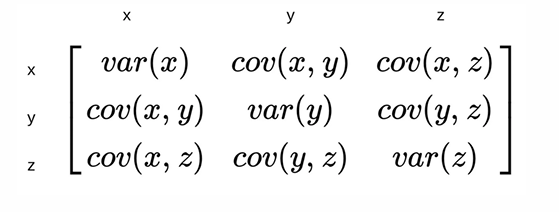
\includegraphics[width=0.5\linewidth]{Images/covmatrix2.png}
    \caption{Example Covmatrix}
\end{figure}

\begin{figure}[H]
    \centering
    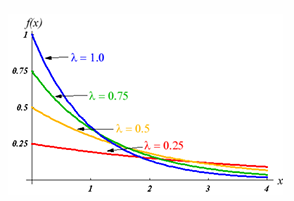
\includegraphics[width=0.5\linewidth]{Images/1func.png}
    \caption{\(\boldsymbol{1}_{x\geq0}\) Function}
\end{figure}

\defn{Exp and Laplace Distribution}{
    \begin{equation}
        p(x;\lambda) = \lambda \boldsymbol{1}_{x \geq 0} exp(- \lambda x)
    \end{equation}
    \begin{itemize}
        \item 1 if the 
        argument (.) is greater or equal zero 
        and zero otherwise.
        \item In other words, for negative values of 
        x, the exponential function is zero
        \item The larger \(\lambda\), the more extreme is the 
        peak at zero
    \end{itemize}

    If the peak should be at an 
    arbitrary point, then the Laplace 
    distribution is helpful:
    \begin{equation}
        Laplace(x; \mu, \gamma) = \frac{1}{2\gamma} exp(- \frac{|x - \mu|}{\gamma})
    \end{equation}
}

\begin{figure}[H]
    \centering
    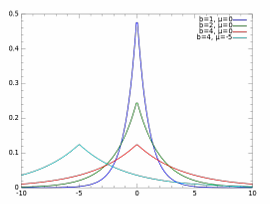
\includegraphics[width=0.5\linewidth]{Images/laplace-d.png}
    \caption{Laplace Distribution: The bigger \(gamma\), the steeper the peek, peak is at \(\mu\)}
\end{figure}

\defn{Dirac}{
    Using a Dirac delta function, it is 
    possible to define pdfs which 
    have a probability greater than 
    zero at one given point.
    \begin{equation}
        p(x) = \delta(x - \mu)
    \end{equation}
}

\begin{figure}[H]
    \centering
    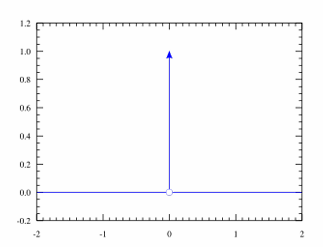
\includegraphics[width=0.5\linewidth]{Images/dirac.png}
    \caption{Dirac Distribution: Arrows shows the functions goes to \(\infty\)}
\end{figure}

\defn{Empirical Distribution}{
    Using dirac delta we can describe density functions using discrete data.
    \textbf{The function is 0 everywhere, except at 0, there it goes to infinity.}
    \begin{equation}
        \hat{p}(\boldsymbol{x}) = \frac{1}{m} \sum_{i=1}^{m} \delta(\boldsymbol{x}-\boldsymbol{x}^{(i)})
    \end{equation}
}

\section{Common Functions}
\defn{Sigmoid}{
    De-Facto standard in binary classification:
    \begin{equation}
        \sigma(x) = \frac{1}{1+ exp(-x)}
    \end{equation}
    \begin{itemize}
        \item Note that for very small and very 
        large value of x, the sigmoid saturates 
        to 0 respectively 1 and the 
        derivatives at those values converge 
        towards 0. This will become a problem later on
    \end{itemize}
}

\begin{figure}[H]
    \centering
    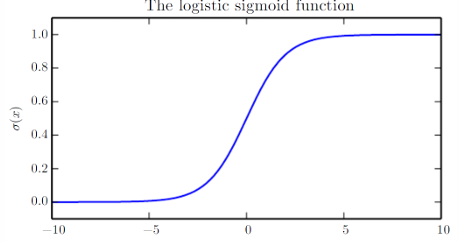
\includegraphics[width=0.5\linewidth]{Images/sigmoid.png}
    \caption{Sigmoid Function}
\end{figure}

\begin{figure}[H]
    \centering
    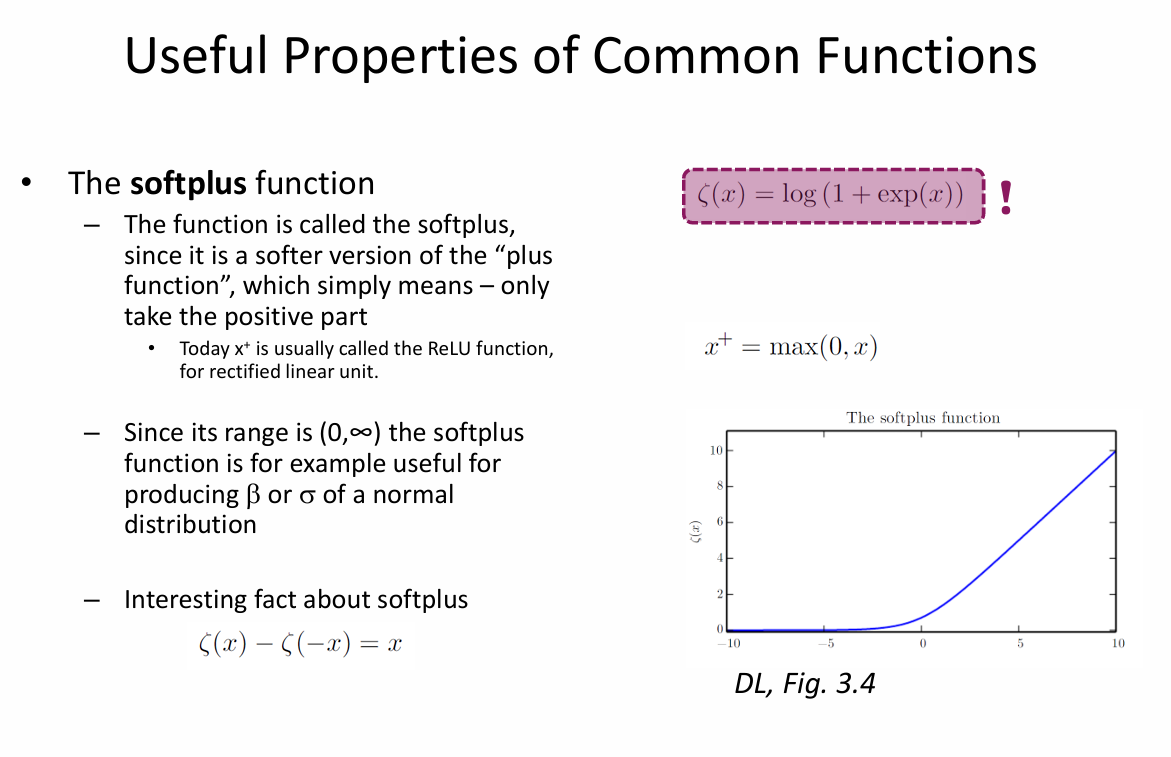
\includegraphics[width=1\linewidth]{Images/relu.png}
    \caption{RELU Function}
\end{figure}

\begin{figure}[H]
    \centering
    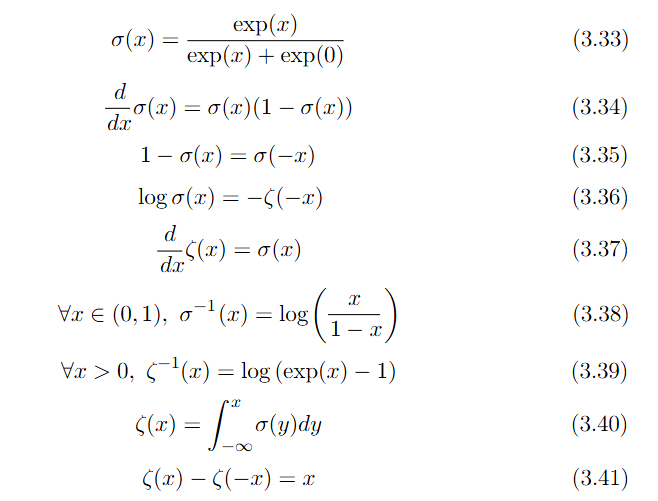
\includegraphics[width=1\linewidth]{Images/comm-useful-props.png}
    \caption{Useful Properties ofCommon Functions}
\end{figure}

\defn{Deterministic Functions of rvs}{
    \begin{equation*}
        \begin{split}
            y = g(x) \\
            p_y(y) \neq p_x(g^{-1}(y))
        \end{split}
    \end{equation*}
    If we now one of the probability densities.
    We cannot just calculate with the invervse function.

    We need to do this:
    \begin{equation}
        \begin{split}
            y = g(x) \\
            | p_y(g(x)) dy | = |p_x(x)dx| \\
            p_y(y) = p_x(g^{-1}(y)) |\frac{\partial x}{\partial y}| \\
            p_x(x) = p_y(g(x)) |\frac{\partial g(x)}{\partial x}|
        \end{split}
    \end{equation}
    This is because g() can warp the space. We need to account for this by looking at a small interval.
}

\defn{Deterministic Functions of multidimensional rvs}{
    \begin{equation}
        \begin{split}
            p_x(x) = p_y(g(x)) | det(\frac{\partial g(x)}{\partial x}) \\
            \text{With Jacobian:} \\
            J = \begin{bmatrix}
                \frac{\partial f_1}{\partial x_1} & \cdots & \frac{\partial f_1}{\partial x_n}\\
                \vdots & \ddots & \vdots\\
                \frac{\partial f_m}{\partial x_1} & \cdots & \frac{\partial f_m}{\partial x_n}
            \end{bmatrix} \\
            \Rightarrow det(J)
        \end{split}
    \end{equation}
    The determinant measures how much g(x) warps the space over which we integrate.
}

\section{Information Theory}
Is a mathematical framework that uses probability theory to describe information.
See lecture Digitale Kodierungen. Any measure of information should satisfy three statements:
\defn{Fundamental Rules}{
    \begin{enumerate}
        \item Likely event should have low information content
        \item Less likely events should have a higher information content
        \item Independent events should have additive information
    \end{enumerate}
}

\defn{Information Content}{
    \begin{equation*}
        I(x) = log(\frac{1}{P(x)}) = -log P(x)
    \end{equation*}
    The base of log is unimportant. It is common to use the natural logarithm to base e.
    This results in the unit called \textit{nats}. In communication theory its common to use base 2.
}


\begin{figure}[H]
    \centering
    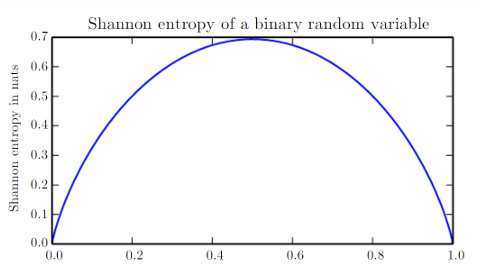
\includegraphics[width=0.75\linewidth]{Images/shannon-entropy.png}
    \caption{Shannon entropy of a binary random variable.
    The x axis shows the argument of the bernoulli distribution.
    The y axis shows the entropy using base e
    If the rv is always zero or one the entropy is also 0. 
    If the rv is completly random (0.5) then the entropy is maximized with 0.7 nats.}
\end{figure}

\defn{Shannon Entropy}{
    Is the \textbf{average information content} over an entire distribution.
    Since it depends on the probability distribution it is commonly written as \(H(P)\).
    The entropy of a distribution is the expected amount of information in
    an event drawn from this distribution.

    \begin{equation}
        H(x) = \mathbb{E}_{x \sim P}[I(x)] = -\mathbb{E}_{x \sim P}[log P(x)]
    \end{equation}

    Using base 2 the entropy describes a lower bound on the number of bits
    needed to encode symbols drawn from distribution p.
}

\defn{Kullback-Leibler (KL) Divergence}{
    Measures different probability distributions P and Q.
    When using base 2 it describes how many additional bits you
    have to send when sending symbols from distribution P with a code 
    designed for distribution Q.

    \begin{equation}
        \begin{split}
            D_{KL}(P||Q) = \mathbb{E}_{x \sim P}[log \frac{P(x)}{Q(x)}] \\
            = \mathbb{E}_{x \sim P}[log P(x) - log Q(x)]
        \end{split}
    \end{equation}

    The divergence is never negative and zero if and only if P and Q are the same.
    The KL divergence is not symmetrical, hence not a distance measure.

    \begin{equation}
        D_{KL}(P||Q) \neq D_{KL}(Q||P)
    \end{equation}

    It can be decomposed:
    \begin{equation}
        \begin{split}
            D_{KL}(P||Q) &= \mathbb{E}_{x \sim P}[log P(x)] - \mathbb{E}_{x \sim P}[log Q(x)] \\
            \text{D} &= \text{Entropy} + \text{Cross-Entropy} \\
            D_{KL}(P||Q) &= -H(x) + H(P,Q)
        \end{split}
    \end{equation}

    If we want to have to similar (or equal) distributions it is feasable to minimize the KL divergence.
    Tho it creates the same solution as minimizing the cross-entropy since only it also depends on Q.

    Important: Assume that \(0 log 0 = 0\)!
}

\begin{figure}[H]
    \centering
    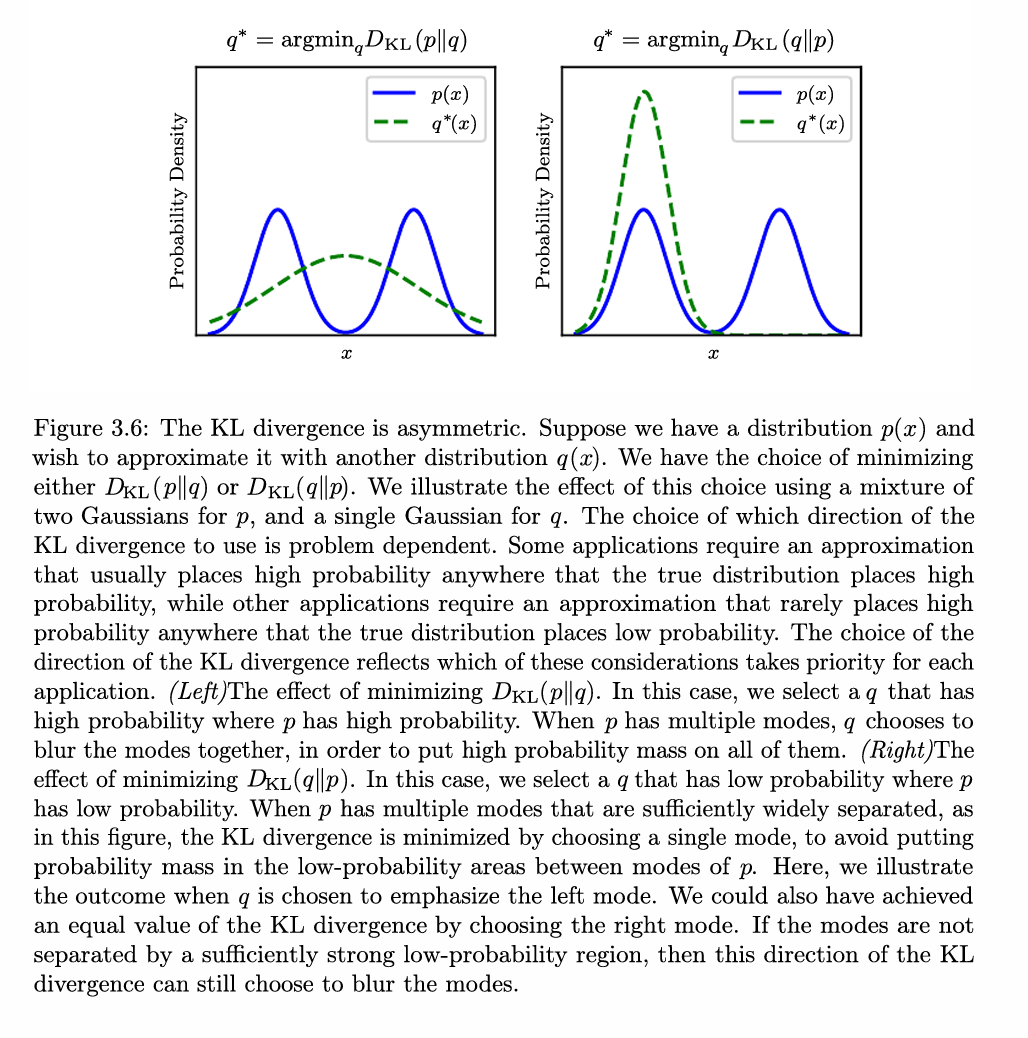
\includegraphics[width=1\linewidth]{Images/kl-divergence-simmetry.png}
\end{figure}

\defn{Cross-Entropy}{
    Measures number of bits (if used with base 2) requirede to send symbols from P
    when using a code designed for distribution Q.

    \begin{equation*}
        H(P,Q) = - \mathbb{E}_{x \sim P}[log Q(x)]
    \end{equation*}

    Minimizing the KL divergence for Q and minimizing the crossentropy for Q are equivalent.
    Vecause shannon entropy does not depend on Q.
}

\subsection{Using KL}
Given some data \(x^{(1)}\) to \(x^{(m)}\) we can write down the empirical data distribution:
\begin{equation*}
    \hat{p}(x) = \frac{1}{m} \sum_{i=1}^{m} \delta (x -x^{(i)})
\end{equation*}
Then we build a prediction model pmodel using a neural network.
The training process aims to make pmodel as similar to \(\hat{p}(x)\).
This can be achieved by minimizing the KL divergence or equivalenty the cross-entropy.

\section{Numerics}


\begin{figure}[H]
    \centering
    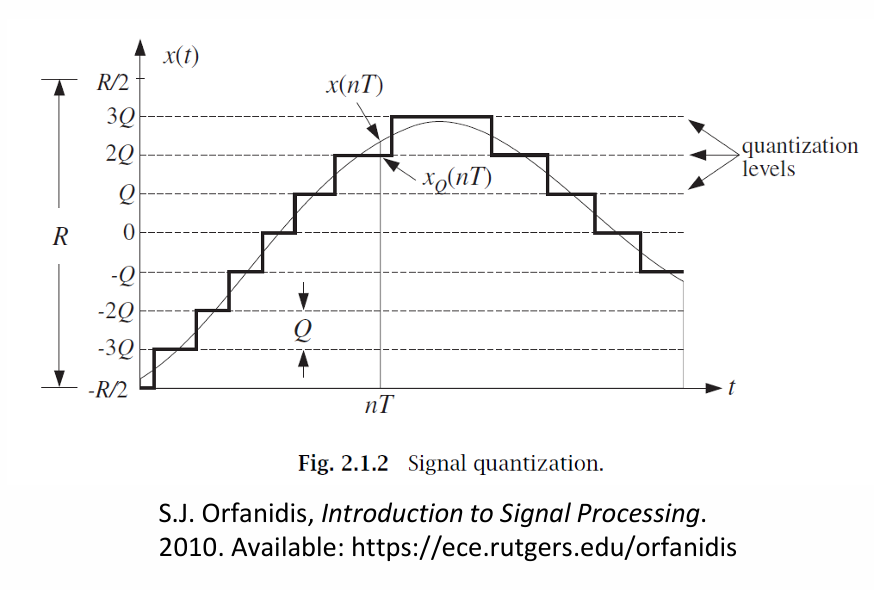
\includegraphics[width=0.75\linewidth]{Images/quantization-error.png}
    \caption{The graph show the q scale on the y axis. Every real values must be mapped to the
    closest quanzitation on the q scale. This results in the stair function approximation of the real function.
    The error depends on the difference between the quantization levels.}
\end{figure}

\defn{Quantization}{
    When using real random variables values from infinite many numbers can appear.
    The fundamental problem lies in the fact that digital computers use bits
    as their numeric representation.

    \begin{itemize}
        \item Hence for almost all real numbers, the digital representation must be an approximation
        \item The error between the real number and its representation is a rounding error
        \item Rounding errors can accumulate over several operations
        \item An algorithm that works in therory might not work on a digital computer since
        it may not be able to minimize the accumulation of errors.
    \end{itemize}

}

\defn{Softmax Function}{
    Is often used as the last layer of a DNN.
    Can convert a vector x into proper class probability. (Following a multinoulli).    

    \begin{equation}
        softmax(x)_i = \frac{exp(x_i)}{\sum_{j=1}^{n} exp(x_j)}
    \end{equation}

    Stabilization in 2 dimensions:
    \begin{equation}
        \begin{split}
            x &= \begin{bmatrix}
                x_1 \\
                x_2
            \end{bmatrix} \\
            softmax(x_1) &= \frac{x_1}{exp(x_1) + exp(x_2)} \\
            &= \frac{exp(x_1 - x2)}{exp(x_1 - x_2) + exp(0)} \\
            \sigma(x) &= \frac{exp(x)}{exp(x)- exp(0)}
        \end{split}
    \end{equation}
    Hence we can stabilize softmax by subtracting the maximum entry of
    the vector x from other entries.
    Subtracting the scalar k does not change the result.
    By subtractng we ensure, that the largest entry is now zero which
    ensures 1 since log(0) = 1. The denominator is also atleast 1.

    Often we take the log of a softmax function. This means when an underflow
    occurs it can lead to \(-\infty\) which is not meaningful.
    Henve most often a log-softmax function is provided by frameworks
    which stabilizes in the same way as the softmax function:
    \begin{equation}
        \begin{split}
            log softmax(x_1) & \Rightarrow \\
            log \frac{exp(x_1)}{exp(x_1)+exp(x_2)} &= log \frac{exp(x_1-x_2)}{exp(x_1-x_2)+exp(0)}\\
            &= log(exp(x_1-x_2)) - log(exp(x_1-x_2)) + exp(0) \\
            &= (x_1-x_2) -log(exp(x_1-x_2)+1)
        \end{split}
    \end{equation}
}

\begin{figure}[H]
    \centering
    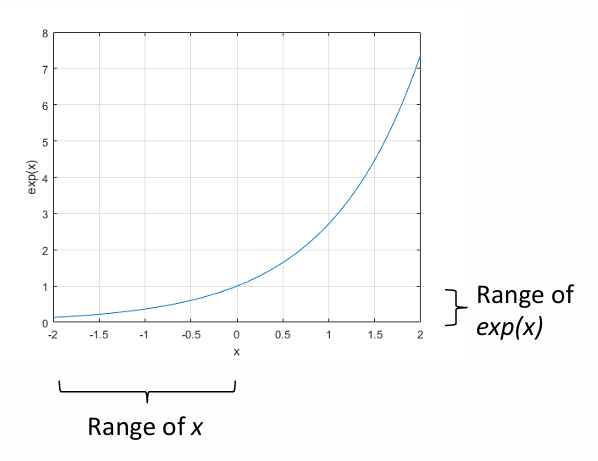
\includegraphics[width=0.75\linewidth]{Images/softmax-stabilization.png}
    \caption{When stabilizing the softmax function the range of x is guaranteed to be negative and exp(x) between 0 and 1.}
\end{figure}

\defn{Poor Conditioning}{
    If a function is poorly conditioned,
    small changes of the input have large effects on the output.
    The system then becomes very sensitive to rounding errors.

    If we assume matrix A has an eigenvalue decomposition, then the
    condition number is defined as:
    \begin{equation}
        \begin{split}
            f(x) &= A^{-1}x \\
            max_{i,j} |\frac{\lambda_i}{\lambda_j}| &= \text{ Condition Number}
        \end{split}
    \end{equation}
    Ratio between the largest and smallest eigenvalue. (Max/Min)

    \begin{itemize}
        \item Well conditioned matrix has condition number a bit larger than 1
        \item Under reasonable assumptions A and \(A^{-1}\) have the same conditioning number
    \end{itemize}
}

\section{Gradient-Based Optimization}
\defn{Learning}{
    \begin{equation}
        \text{Learning } = \text{ Minimizing a Loss Function}
    \end{equation}
    Optimization algorithms that use only the gradient are called \textbf{first-order optimization algorithms}.
}

\defn{Loss function}{
    The loss function is given as
    f(x) where x is a vector of all learnable parameters.
    Typically in dl we use the Kullback-Leibler Divergence
    between the empirical distribution and the model distribution
    as loss function.

    The optimal value that minimizes the function is denoted as \(x^*\):
    \begin{equation}
        \boldsymbol{x}^* = arg min f(\boldsymbol{x})
    \end{equation}
}
\begin{figure}[H]
    \centering
    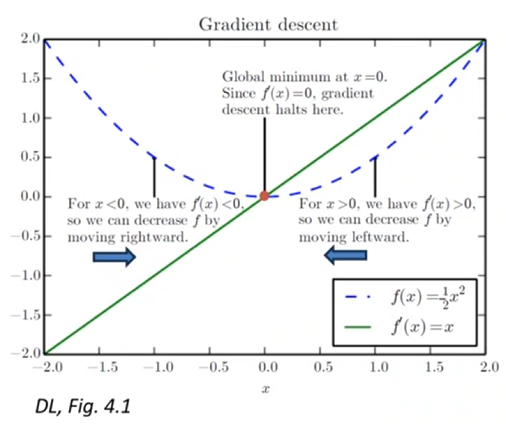
\includegraphics[width=0.75\linewidth]{Images/gradient-descent.png}
    \caption{Gradient Descent}
\end{figure}

\begin{figure}[H]
    \centering
    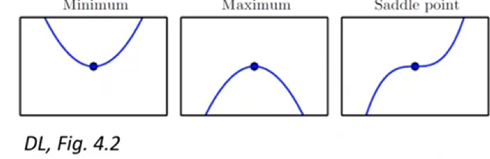
\includegraphics[width=0.75\linewidth]{Images/stationary-points.png}
    \caption{Stationary Points. Include global and local minima and maxima as well as saddle points}
\end{figure}

\begin{figure}[H]
    \centering
    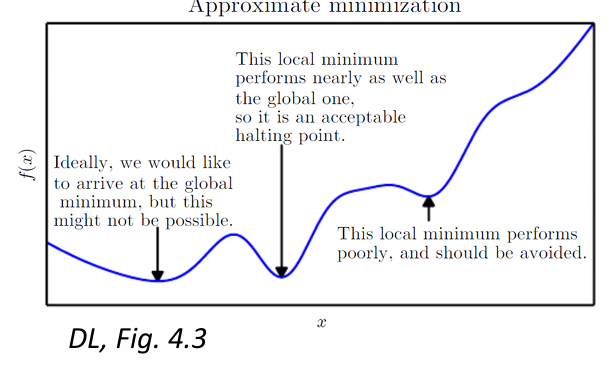
\includegraphics[width=0.75\linewidth]{Images/minimas.png}
    \caption{Graph showing function with multiple minima}
\end{figure}

\defn{Directional Derivative}{
    At some point x the directional derivative,
    is the derivative in direction unit vector u.
    \begin{equation}
        \frac{\partial}{\partial \alpha} f(\boldsymbol{x} + \alpha \boldsymbol{u}) = \boldsymbol{u}^T \nabla_x f(\boldsymbol{x}), \text{ at } \alpha = 0
    \end{equation}
}

\begin{figure}[H]
    \centering
    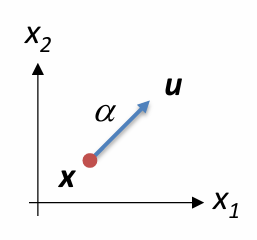
\includegraphics[width=0.25\linewidth]{Images/directional-derivative.png}
    \caption{Directional derivative}
\end{figure}

\defn{Gradient Descent (Steepest Descent)}{
    \begin{equation}
        \begin{split}
            f: \mathbb{R}^n &\to \mathbb{R} \\
            \text{with } \frac{\partial}{\partial \alpha} f(\boldsymbol{x} + \alpha \boldsymbol{u}) &= \boldsymbol{u}^T \nabla_x f(\boldsymbol{x}), \text{ at } \alpha = 0 \\
            &\Rightarrow \\
            &min_{u,u^T|u=1} \boldsymbol{u}^T \nabla_x f(\boldsymbol{x}) \\
            &= min || \boldsymbol{u} ||_2 || \nabla_x f(x) ||_2 cos \theta \\
            &\Rightarrow min_u cos \theta
        \end{split}
    \end{equation}
    Minimizing theta range (-1 to 1) evaluates to cos theta = -1:
    \begin{equation}
        \boldsymbol{x}' = \boldsymbol{x} - \varepsilon \nabla_x f(\boldsymbol{x})
    \end{equation}

    There are many schemes to pick \(\varepsilon\):
    \begin{itemize}
        \item Set it to small value (popular)
        \item Search along negative gradient
        \item Several values and compare loss function
        \item More schemes TBD
    \end{itemize}
}

\defn{Jacobian}{
    \begin{equation}
        \begin{split}
            \text{For } f:R^n &\to R^m \\
            (J_f (x))_{i,j} &= \frac{\partial}{\partial x_j} f_i (x) \\
            J_{f \circ g} (x) &= J_f (g(x)) \cdot J_g (x) \\
            \text{For surfaces applies gradients which basically is a jacobian } s: R^n &\to R \\
            J_s (x)\approx \nabla s &=(\frac{\partial}{\partial_{x_1}} f(x),\cdots,\frac{\partial}{\partial_{x_n}})
        \end{split}
    \end{equation}

    \begin{equation*}
        J_{\text{Example}} = \begin{bmatrix}
            \frac{\partial f_1}{\partial x_1} & \frac{\partial f_1}{\partial x_2} \\
            \frac{\partial f_2}{\partial x_1} & \frac{\partial f_2}{\partial x_2}
        \end{bmatrix}
    \end{equation*}
    Gradient:
    \begin{itemize}
        \item Is perpendicular to contour surfaces of f(x)
        \item Points into direction of steepest ascent
        \item Norm is proportional to steepness
    \end{itemize}
    \begin{equation*}
        \nabla s(g(x)) = \nabla s(u) \cdot J_g(x) \text{ where } g: \mathbb{R}^m \to \mathbb{R}^n
    \end{equation*}
}

\defn{Hessian}{
    Is the second order derivative of vector valued functions.
    \begin{equation*}
        \begin{split}
            f: \mathbb{R}^n \to \mathbb{R} \\
            (H_f (x))_{i,j} &= \frac{\partial}{\partial x_i} \frac{\partial}{\partial x_j} f (x) \\
        \end{split}
    \end{equation*}
    It can describe how much a function "bends", the curvature.
    If the curvature is zero, then the slope does not change, hence the function is a line, plane or hyperplane.
    \begin{itemize}
        \item Is the jacobian of the gradient of f(x)
        \item Anywhere that the second partial defivatives are continuous, the differential operators are \textbf{commutative}
        \item Usually for the functions we encounter the Hessian is \textbf{symmetric}.
        \item If the Hessian is real and symmetric, it can be decomposed into a set of Eigenvalues and orthogonal eigenvectors.
    \end{itemize}
}

For quadratic functions, the curvature tells us:
\begin{table}[H]
    \begin{tabular}{l|l|l}
     Curvature & Slope & Gradient Descent Step  \\
     \hline \\
     Negative & gets smaller & too small  \\
     Zero & stays constant & just right  \\
     Positive & gets larger & too large
    \end{tabular}
\end{table}
Many functions can be well approximated as quadratic functions in a small local neighborhood.

\begin{figure}[H]
    \centering
    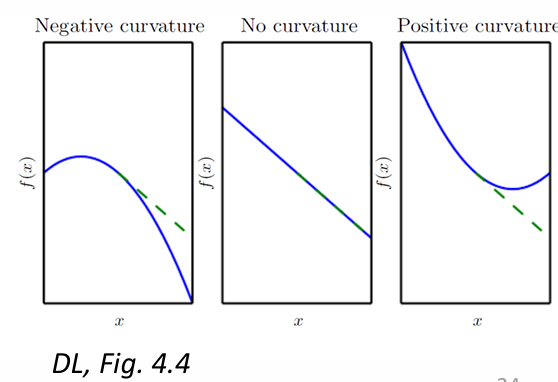
\includegraphics[width=0.5\linewidth]{Images/hessian.png}
    \caption{Curvature with the hessian}
    \label{fig:hessian-curvature}
\end{figure}

\defn{Eigendecomposition of the Hessian}{
    The hessian contains a large number of values, to analyze it more easily, the Eigenvalues are analyzed.

    The second derivative in a direction by unit vector d is given by:
    \begin{equation}
        d^T H d
    \end{equation}

    If d is a unit eigenvector of H then:
    \begin{equation}
        d^THd = d^T \lambda d = \lambda d^T d = \lambda
    \end{equation}

    The second directional derivative in direction of an eigenvector is the corresponing eigenvalue.
    For other directions, it is a weighted average of all eigenvalues.
    The maximum eigenvalue determines the maximum second derivative and the minimum vice versa.

    \textbf{Now instead of looking in any arbritary direction we can analyze the directions of the eigenvectors.
    The curvature there is the corresponding eigenvalue.}

    \begin{equation}
        \begin{split}
            d^T H d \text{ with } H=V \Lambda V^T \\
            = d^T V \Lambda V^T d = \sum_{i} (d^T v_i)^2 \lambda_i \\
            = \sum_{i} (cos \theta_i)^2 \lambda_i
        \end{split}
    \end{equation}
    This is a sum over all i's eigenvalue/vector pairs, with the cosine between the angles of the directions
    multiplied the corresponding eigenvalue.
    \textbf{For any direction we can calculate the curvature based on this linear combination.}
}

\defn{Second order Taylor approximation}{
    Locally approximates a function f(x)
    around a given point x(0) using gradient g and Hessian H.

    \begin{equation}
        f(x) \approx f(x^{(0)}) + (x-x^{(0)})^T g + \frac{1}{2}(x-x^{(0)})^T H(x-x^{(0)})
    \end{equation}

    The approximated value after one step of the gradient descent is then:
    \begin{equation}
        \begin{split}
            x^{(0)} - \alpha g \\
            = f(x^{(0)} - \alpha g) \approx f(x^{(0)}) - \alpha g^T g + \frac{1}{2} \alpha^2 g^T H g
        \end{split}
    \end{equation}
    The first to parts do not contribute to the analysis for the minimization problem.
    For the last part:
    \begin{equation}
        \frac{1}{2} \alpha^2 g^T H g
    \end{equation}
    See figure \ref{fig:hessian-curvature} on page \pageref{fig:hessian-curvature}.
    The sign of the part tells us:
    \begin{description}
        \item[Negative] Negative curvature
        \item[Zero] No curvature
        \item[Positive] Positive curvature;
        This is an optimization problem since, we might end up in the wrong place due to the curve change,
        hence the optimization will fail.
    \end{description}
    When this i positive, we can theoretically calculate for the optimal \(\epsilon \text{ respectively } \alpha\):
    \begin{equation}
        \alpha^* = \frac{g^T g}{g^T H g}
    \end{equation}
}

For critical points in multiple dimensions:
\begin{equation*}
    \nabla_x f(x) = 0
\end{equation*}
We can judge it in analogy to the second order derivative in one dimension:
\begin{table}[H]
    \begin{tabular}{l|l|l}
     Type of critical point & Eivenvalues of H & 2nd order directional derivatives  \\
     \hline \\
     Minimum & All positive & Positive in all possible directions  \\
     Maximum & All negative & Negative in all possible directions  \\
     Saddle point & Some positive, some negative & Positive in some, negative in other directions
    \end{tabular}
\end{table}


\defn{Second Order Condition Numbers}{
    The condition number of the Hessian is a good way of measuring how much the second derivatives vary
    as seen in figure \ref{fig:hessian-condition-number}.
    \begin{itemize}
        \item A small condition means curvature is similar in all directions, hence we use a large step size.
        \item A high condition number means large curvature in one and small in another direction.
        A small step size is needed to prevent overshooting in one direction. This means slow progress in other directions.
    \end{itemize}
}

\begin{figure}[H]
    \centering
    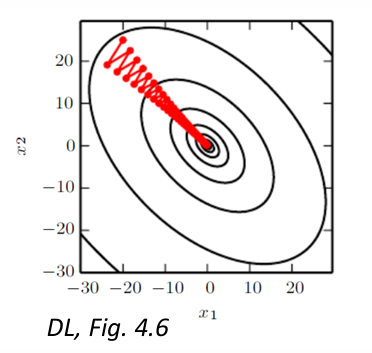
\includegraphics[width=0.5\linewidth]{Images/hessian-conditioning.png}
    \caption{Condition Number using the Hessian}
    \label{fig:hessian-condition-number}
\end{figure}

\defn{Newtons Method}{
    Can be used iteratively using the second order for minimizing a function(x).
    We can analytically find the minimum of e.g a quadratic function:
    \begin{equation}
        x^* = x^{(0)} - H(f)(x^{(0)})^{-1} \nabla_x f(x^{(0)})
    \end{equation}
    This requires the inverse of the Hessian which is unreasonable in high dimensional spaces.

    This comes from the second order taylor approximation:
    \begin{equation*}
        f(x^{(0)} - \epsilon g) \approx f(x^{(0)}) - \epsilon g^T g + \frac{1}{2} \epsilon^2 g^T H g
    \end{equation*}
    Where g is the gradient and H the Hessian.
}

\section{Machine Learning}

\defn{ML Algorithm}{
    A machine learning algorithm improves a computers
    performance \textbf{P} at some task \textbf{T} via experience \textbf{E}.

    Usually:
    \begin{itemize}
        \item Task T is predicting y based on x
        \item Experience E is the training data
        \item Performance P is a measurement like the test MSE
    \end{itemize}
}

Tasks T:
\begin{itemize}
    \item Classification 
        \begin{itemize}
            \item Model assigns a Class using \(f : \mathbb{R}^n \to {1,\dots,k}\)
            \item Model outputs probability distribution over classes. 
        \end{itemize}
    \item Classification with missing inputs
        \begin{itemize}
            \item No guarantees that all inputs are available
            \item When some of the inputs may be missing,rather than providing a single classification function,
            the learning algorithmmust learn a set of functions.
            Each function corresponds to classifyingxwitha different subset of its inputs missing.
            \item One way to effciently define such a large set of functions is to learn a probability distribution
            over all the relevant variables, then solve theclassification task by
            marginalizing out the missing variables.
            \item program needsto learn only a single function describing the joint probability distribution
        \end{itemize}
    \item Regression
        \begin{itemize}
            \item \(\mathbb{R}^n \to \mathbb{R}\)
        \end{itemize}
    \item Transcription
        \begin{itemize}
            \item Unstructured representation into discrete textual form
        \end{itemize}
    \item Machine translation
    \item Structured output
        \begin{itemize}
            \item Any task where output is a vector with important relationships between values
            \item subsumes the transcription and translation tasks
        \end{itemize}
    \item Anomaly detection
        \begin{itemize}
            \item E.g detect action / data comming from a different probability distribution
        \end{itemize}
    \item Synthesis and sampling
        \begin{itemize}
            \item enerate new examples that are similar
        \end{itemize}
    \item mputation of missing values
    \item Denoising
    \item Density estimationorprobability mass function estimation
\end{itemize}
Of course, many other tasks and types of tasks are possible.

Performance Measure P:
\begin{itemize}
    \item Classification
        \begin{itemize}
            \item Accuracy and Error-Rate
            \item 0-1 Loss (Error-Rate)
        \end{itemize}
    \item Density Estimation
        \begin{itemize}
            \item average log-probability the model assigns to some samples
        \end{itemize}
\end{itemize}
he choice of performance measure may seem straightforward
and objective, but it is often difficult to choose a performance 
measure that corresponds well to the desired behavior of the system.

\defn{Bias Term}{
    Is not about a statistical bias but rather refers to the intercept term.
    When using a linear function it is strictly speaking a affine function.
    \begin{itemize}
        \item One approach to integrate b is to extend the x vector by one dimension and setting it to 1.
    \end{itemize}
}

\defn{i.i.d Assumption}{
    \begin{itemize}
        \item Why is it ok to train on the MSEtrain when we actually want a small MSE test?
    \end{itemize}

    All samples of the training set and 
    test set are independently and identically distributed, 
    i.e., are generated with the same 
    distribution.

    \begin{equation}
        \mathbb{E}[MSE_{train}] = \mathbb{E}[MSE_{test}]
    \end{equation}
}

\defn{Goal of Machine Learning}{
    Is to perform well on new data.
    Therefore a good generalization results in low test (generalization) error.
    The test error is usually estimated by 
    measuring the performance over a test set 
    of examples.
    \begin{itemize}
        \item  For this to work, the training set and the test set must come from the same data generating process.
    \end{itemize}

    \begin{enumerate}
        \item Train MSE small
        \begin{itemize}
            \item If not achieved: underfitting
        \end{itemize}
        \item Keep gap between MSE train and test small
        \begin{itemize}
            \item If not achieved: overfitting
        \end{itemize}
    \end{enumerate}
}

\begin{figure}[H]
    \centering
    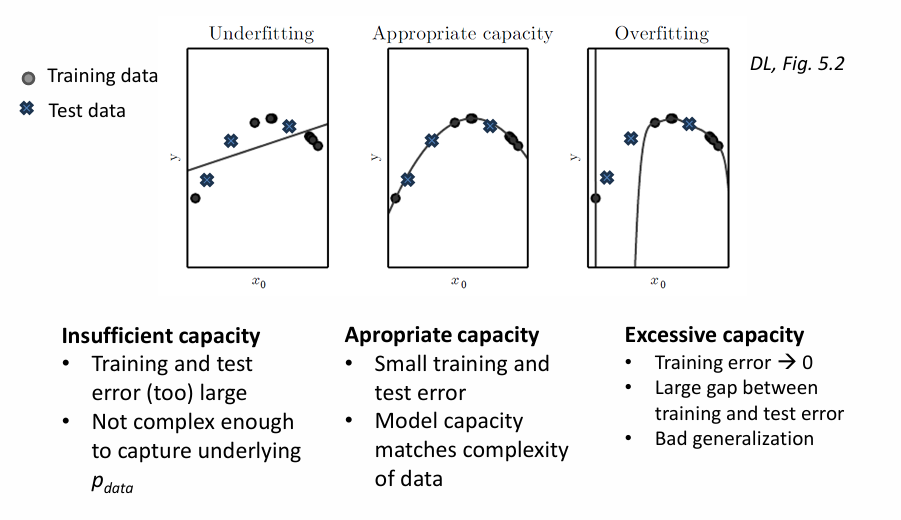
\includegraphics[width=0.75\linewidth]{Images/over_underfitting.png}
    \caption{Overview: Over and Underfitting}
\end{figure}

\defn{Capacity}{
    Is loosely defined as the \textbf{flexibility} of a model to fit to data.
}

\begin{figure}[H]
    \centering
    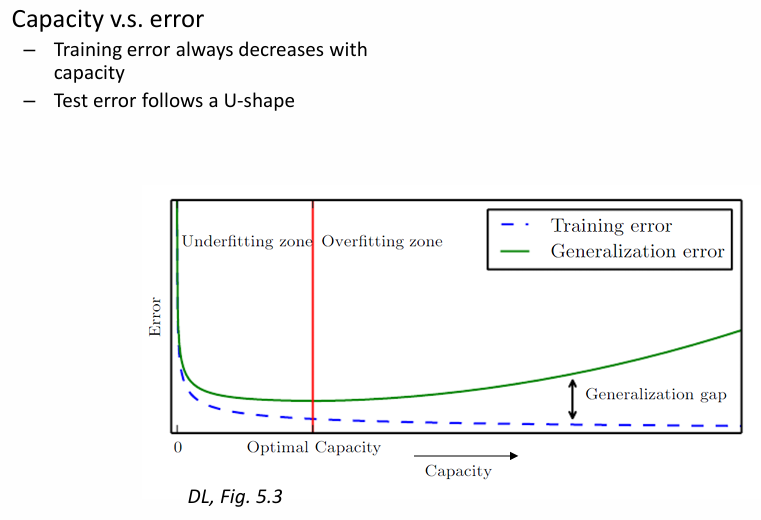
\includegraphics[width=0.75\linewidth]{Images/cap-vs-error.png}
    \caption{Capacity vs Error}
\end{figure}

\defn{Bayes Error (Irreducible)}{
    The smallest possible error is called Bayes or irreducible error.
    It arises from the fact that even if we would know the true data generation distribution
    the underlying process could be inherently stochastic or that it depends on variables not in the input.
}

\defn{No Free Lunch Theorem}{
    No machine learning algorith is universally better than any other.
    \begin{itemize}
        \item Deterministic View
        \begin{itemize}
            \item Logic rules
            \item To create a rule about some data point, we must know that point.
            \item We cannot create deterministic rules based on a small training dataset.
        \end{itemize}
        \item \textbf{Probabilistiv View}
        \begin{itemize}
            \item Probabilistic Rules
            \item Rules which are probably correct for most data points
            \item We can infer these rules based on a small training set
            \item The only option for ML!
        \end{itemize}
    \end{itemize}

    Averaged over all possible data generating distributions, every
    classification algorithm has the same error rate when classifying
    previously unobserved points.
    \begin{itemize}
        \item We can find the optimal algorithm for our problem
    \end{itemize}
}

\defn{Regularization}{
    Regularization is any modification we make to a learning 
    algorithm that is intended to reduce its generalization 
    error but not its training error.

    This is generally achieved by adding a \textbf{penalty term} called \textbf{regularizer} to the cost function.
}

\defn{Hyper-Parameters}{
    Hyperparameters are parameters 
    of a learning algorithm that are 
    not learned by the scheme.

    The \textbf{training set cannot be used}, 
    since changing hyperparameters that 
    increase capacity will always reduce 
    the training error.
    The test set is used to estimate the 
    generalization error, \textbf{we are not allowed} to 
    use it to adjust the hyperparameters.

    \begin{itemize}
        \item \textbf{validation set} (e.g 20\% of training)
    \end{itemize}
}

\defn{Estimators}{
    Statistical estimators introduce the terms bias and variance.
    \begin{itemize}
        \item ML is an estimation process too.
        \begin{itemize}
            \item  Instead of estimating a sample mean, we 
            estimate the parameters of a model.
        \end{itemize}
    \end{itemize}
    The goal of point estimates is, to 
    provide a best estimate of some 
    quantity of interest:
    \begin{equation}
        \begin{split}
            \text{True value of parameter } &\theta \\
            \text{Estimate } &\hat{\theta}
        \end{split}
    \end{equation}

    Point Estimator:
    \begin{equation}
        \hat{\theta}_m = g(x^{(1)}, \cdots, x^{(m)})
    \end{equation}
}

\defn{Bias}{
    \begin{equation}
        bias(\hat{\theta}_m) = \mathbb{E}(\hat{\theta}_m) - \theta
    \end{equation}
    Estimators are considered unbiased, 
    if the bias is zero, which implies that 
    on average the estimator is correct.

    A milder form is the idea of 
    asymptotically unbiased, which 
    means as we gather more and more 
    data, the estimator becomes less and 
    less biased:
    \begin{equation}
        \lim_{m \to \infty} \mathbb{E}(\hat{\theta}_m) = \theta
    \end{equation}
}

\begin{figure}[H]
    \centering
    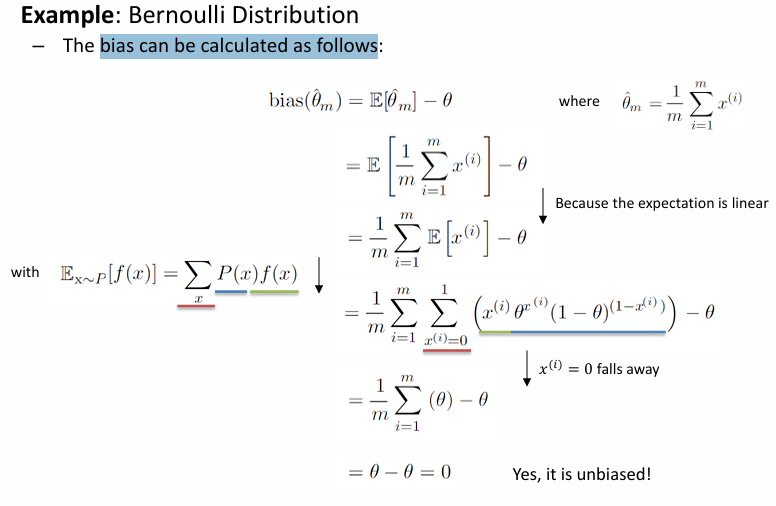
\includegraphics[width=0.75\linewidth]{Images/bias-est-bernoulli.png}
    \caption{Estimator Bias of Bernoulli Parameter}
\end{figure}

\begin{figure}[H]
    \centering
    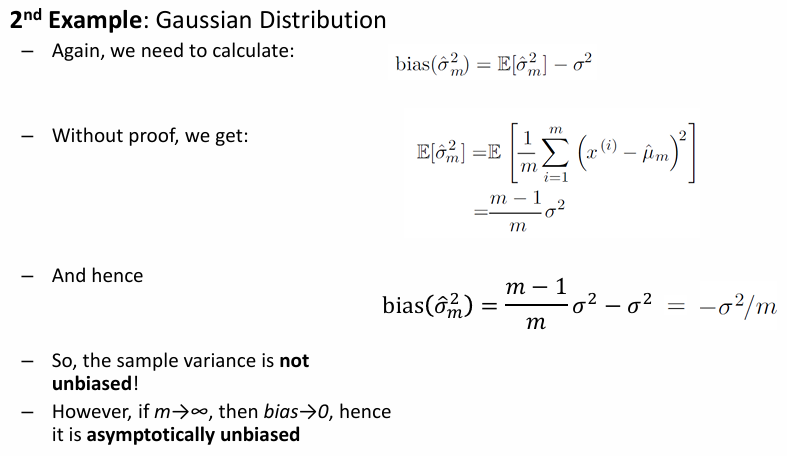
\includegraphics[width=0.75\linewidth]{Images/bias-est-gauss.png}
    \caption{Estimator Bias of Gauss Parameter Sigma}
\end{figure}

In both bias and variance, you assume that you 
repeatedly collect new datasets, 
estimate the parameter on each 
dataset, and monitor the estimate.

\defn{Consistency}{
    Consistency combines the 
    concepts of Bias and Variance.

    A consistent estimator will 
    converge towards the value it 
    tries to estimate, when the 
    available data set converges 
    towards infinity.

    \begin{equation}
        \lim_{m \to \infty} \hat{\theta}_m \to^p \theta
    \end{equation}

    \begin{itemize}
        \item (Asymptotic) unbiasedness
        \item Variance decreased with increasing number of observation
    \end{itemize}
}

\defn{MSE}{
    On a theoretical basis, the mean 
    square error (MSE) of the estimates 
    is defined as:
    \begin{equation}
        \begin{split}
            MSE &= \mathbb{E}[(\hat{\theta}_m - \theta)^2] \\
            &= Bias(\hat{\theta}_m)^2 + Var(\hat{\theta}_m)
        \end{split}
    \end{equation}
}

\begin{figure}[H]
    \centering
    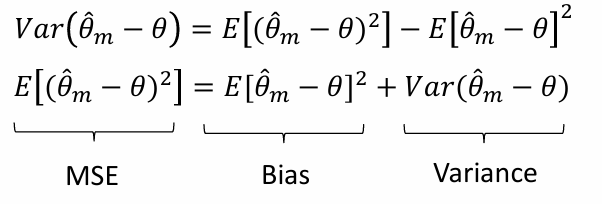
\includegraphics[width=0.75\linewidth]{Images/mse-bias-variance.png}
    \caption{MSE Bias and Variance}
\end{figure}

\begin{figure}[H]
    \centering
    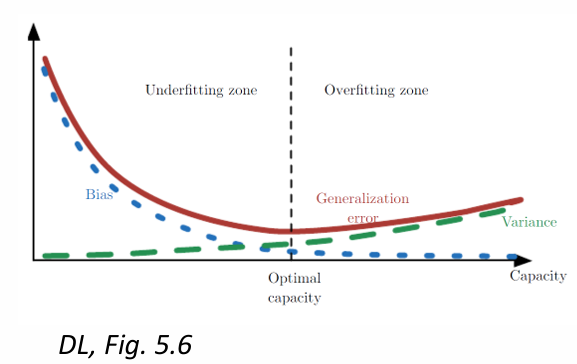
\includegraphics[width=0.75\linewidth]{Images/mse-bias-variance-tradeoff.png}
    \caption{MSE Bias and Variance Tradeoff}
\end{figure}

\defn{Maximum Likelihood Estimation}{
    Method to find good estimators.
    Given an \textbf{i.i.d dataset} with m examples
    from an unkown data generating distribution:
    \begin{equation*}
        \mathbb{X} = \{x^{(1)},\dots,x^{(m)}\}
    \end{equation*}

    Our goal is to estimate the 
    unknown \(p_{data}(x)\) based on the 
    observed data.

    We define some parametric model distribution:
    \begin{equation*}
        p_{model}(x,\theta)
    \end{equation*}

    Now we try to find the parameter 
    vector \(\theta\) that results in the largest
    likelihood of having generated our
    measured data. Hence, we maximize the likelihood:
    \begin{equation*}
        \hat{\theta}_{ML} = {\text{arg max}}_{\theta} p_{model}(\mathbb{X};\theta)
    \end{equation*}
    This is called "parametric estimation".

    Because we assume it is i.i.d. we can decompose into:
    \begin{equation*}
        {\text{arg max}}_{\theta} p_{model}(\mathbb{X};\theta) = {\text{arg max}}_{\theta} \prod_{i=1}^{m} p_{model}(x^{(i);\theta})
    \end{equation*}
    And transform it into a sum:
    \begin{equation*}
        {\text{arg max}}_{\theta} \sum_{i=1}^{m} \log p_{model}(x^{(i);\theta})
    \end{equation*}

    We describe the observed data with an empirical
    distribution, which is given by (\(\frac{1}{m}\) does not change resulting \(\theta\)):
    \begin{equation*}
       \hat{p}_{data}(x) = \frac{1}{m}\sum_{i=1}^{m} \delta (x-x^{(i)})
    \end{equation*}

    This means the likelyhood closely resembles the structure of the Expectation of a function
    applied to x following a model emprirical distribution:
    \begin{equation*}
        \mathbb{E}_{x \sim \hat{p}_{data}} f(x) = \frac{1}{m} \sum_{i=1}^{m} f(x^{(i)})
    \end{equation*}

    This means the maximum likelyhood estimation is equivalent to:
    \begin{equation}
        \begin{split}
            =  &{\text{arg max}}_{\theta} \mathbb{E}_{x \sim \hat{p}_{data}} \log p_{model}(x;\theta) \\
            &H(P,Q) = -\mathbb{E}_{x \sim P} \log Q(x)
        \end{split}
    \end{equation}

    \textbf{Maximum likelihood estimation is equivalent to minimizing the cross-entropy 
    between the empirical distribution and the model distribution}.

    \begin{equation}
        \hat{\theta}_{ML} = {\text{arg min}}_{\theta} H(\hat{p}_{data}, p_{model})
    \end{equation}
}


Maximum likelihood estimation 
can be interpreted as making the 
model distribution match the 
empirical distribution.

We would rather match the true data 
generating distribution, but we have 
no direct access to this distribution.

\defn{Max Likelihood and KL-Divergence}{
    Since the first part of Kullback-Leibler divergence does not depend on the model,
    minimizing the cross-entropy is equivalent to minimizing the KL-divergence, hence
    minimizing KL-divergence leads to a maximum likelihood estimate.
    \begin{equation*}
        D_{KL} = (\hat{p}_{data} || p_{model}) = \mathbb{E}_{x \sim \hat{p}_{data}}[\log \hat{p}_{data}(x) - \log p_{model}(x)]
    \end{equation*}
    \begin{equation}
        \hat{\theta}_{ML} = {\text{arg min}}_{\theta} D_{KL}(\hat{p}_{data} || p_{model})
    \end{equation}
}

\defn{Conditional Log-Likelihood}{
    In supervised learning we need to estimate the conditional probability:
    \begin{equation*}
        p_{model}(x;\theta) \to P(y | x;\theta)
    \end{equation*}
    Where X is a matrix containing measured input (design matrix) and Y containing all measured outputs.
    \begin{equation*}
        \hat{\theta}_{ML} = {\text{arg max}}_{\theta} P(y | x;\theta)
    \end{equation*}
    \begin{equation}
        \hat{\theta}_{ML} = {\text{arg max}}_{\theta} \log P(y^{(i)} | x^{(i)};\theta)
    \end{equation}
}

\begin{figure}[H]
    \centering
    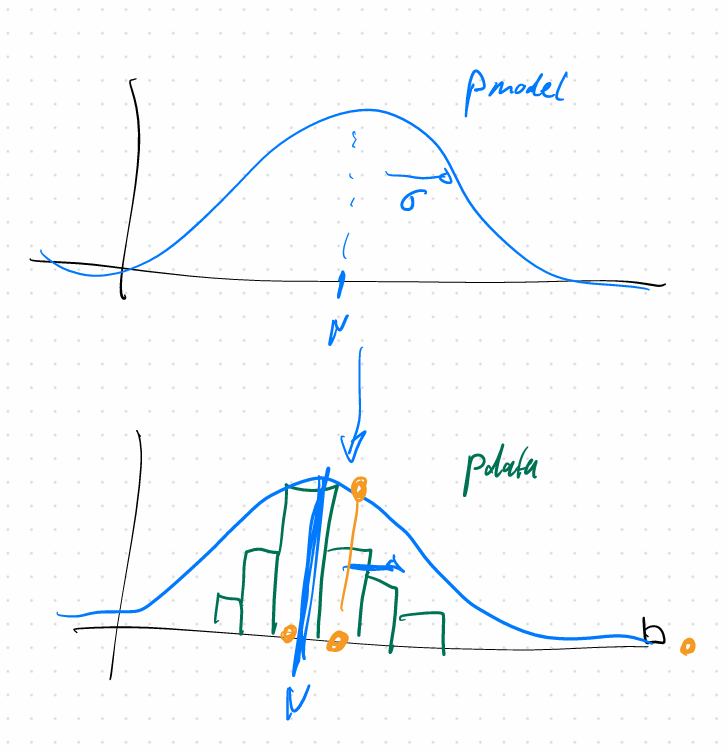
\includegraphics[width=0.75\linewidth]{Images/estimation-pmodel.png}
    \caption{We use a gaussian model which we want to fit to our empirical distribution.
    When using "better" parameters of the gaussian model the fit measured in the maximum likelyhood aproaches 1.
    Meaning samples of the underlying empirical distribution are likely to appear in our model distribution.}
\end{figure}

\begin{figure}[H]
    \centering
    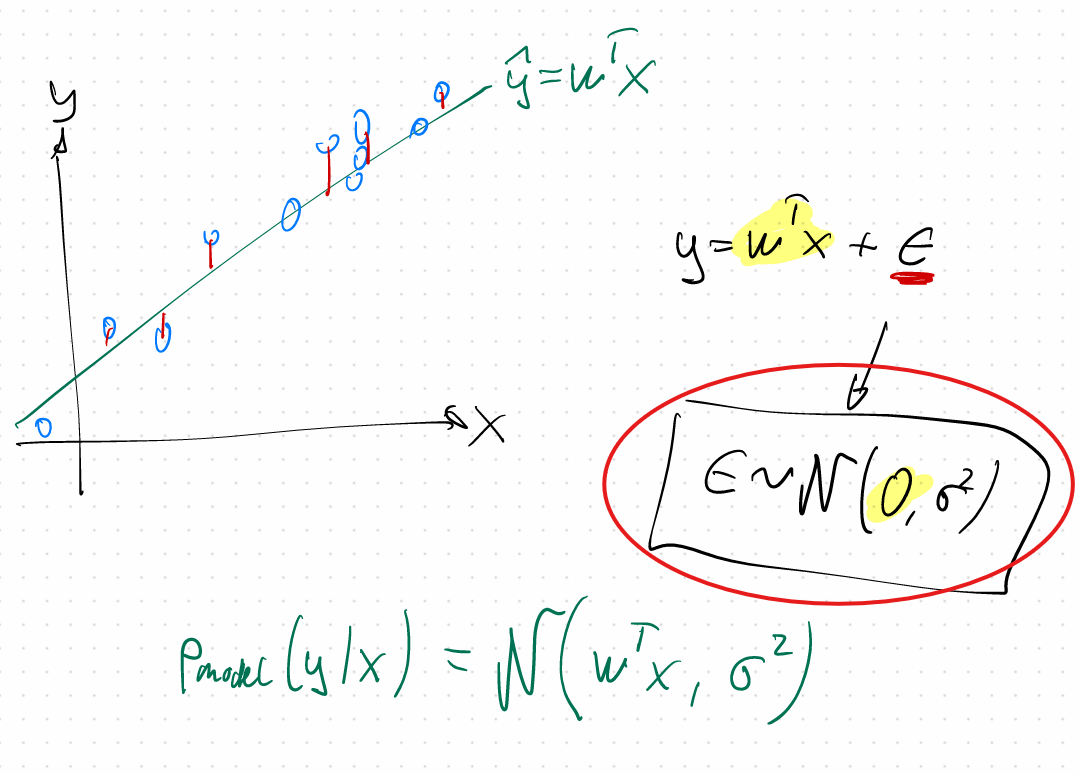
\includegraphics[width=0.75\linewidth]{Images/linear-regression-assumption.png}
    \caption{For linear regression we include probabilistic error in our model, converting it into a
    probabilistic model. For this we assume e.g that the error mean is zero (resp. is around y) but with an unkown variance.}
\end{figure}

\defn{Linear Model in Conditional Log-Likelihood}{
    We assume:
    \begin{itemize}
        \item Model is on average correct
        \item There is a remaining random error, which follows a gaussian
        \item We assume a \textbf{constant} variance e.g 1 since we don't know the true variance (this does not matter later on)
    \end{itemize}
    \begin{equation}
        p(y|x) = N(y; \hat{y}(x;w),\sigma^2)
    \end{equation}

    If we now rewrite the log likelihood as shown in figure \ref{fig:linear-regression-loglikelihood} on page
    \pageref{fig:linear-regression-loglikelihood} we can find that this is equvalent to minimizing the MSE.

    \textbf{Hence, minimizing MSE is a maximum likelihood estimate under the assumption 
    that the errors follow a Gaussian distribution.}
}

\begin{figure}[H]
    \centering
    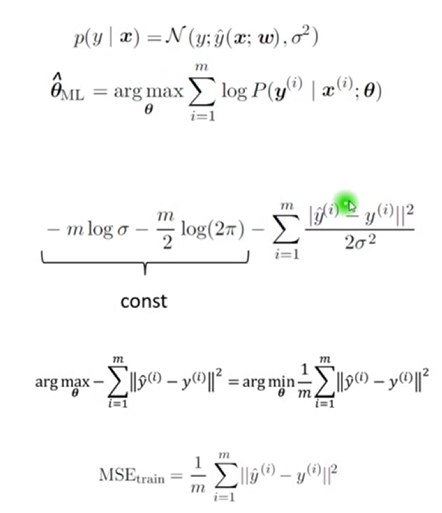
\includegraphics[width=0.6\linewidth]{Images/linear-regression-loglikelihood.png}
    \caption{If we plug in the linear probabilistic model into the conditional log likelihood,
    we will get the minimization of the MSE as a result}
    \label{fig:linear-regression-loglikelihood}
\end{figure}

\defn{Stochastic Gradient Descent}{
    When training neural networks using Maximum Likelihood and
    a gradient based approach, we require the gradient.
    This requires the gradient calculation over all training data which can be slow.
    
    We can use SGD to solve this problem.
    For this we decompose the max likelihood problem as seen in figure \ref{fig:decomposition-maxlikelihood-sgd}
    on page \pageref{fig:decomposition-maxlikelihood-sgd}.

    When calculating the gradient of loss function J we can show that this is also an expectation:
    \begin{equation*} 
        \begin{split}
            \nabla_\theta J(\theta) &= \frac{1}{m} \sum_{i=1}^{m} \nabla_\theta L(x^{(i)},y^{(i)},\theta) \\
            \nabla_\theta J(\theta) &= \mathbb{E}_{x,y \sim \hat{p}_{data}}[\nabla_\theta L(x,y,\theta)]
        \end{split}
    \end{equation*}

    Key idea: an expectation can be estimated with any number m' of data samples:
    \begin{equation}
        \hat{g} = \frac{1}{m'} \sum_{i=1}^{m'} \nabla_\theta L(x^{(i)},y^{(i)},\theta)
    \end{equation}

    In each step of SGD, a so called 
    \textbf{minibatch} \(\mathbb{B}\) of samples is used, 
    where the m' samples are drawn randomly from the training set.
}

\begin{figure}[H]
    \centering
    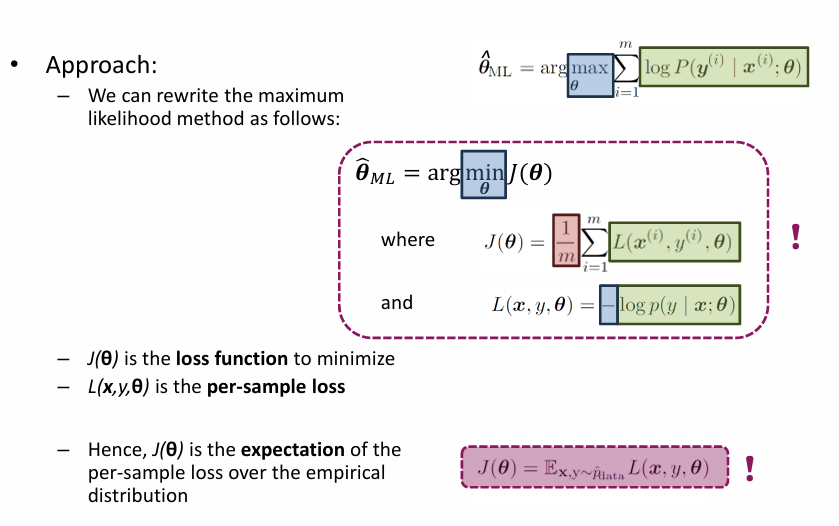
\includegraphics[width=0.75\linewidth]{Images/sgd-rewrite.png}
    \caption{We decompose the Log Likelihood for SGD in multiple components}
    \label{fig:decomposition-maxlikelihood-sgd}
\end{figure}

\section{Building an ML Algorithm}

\subsection{Requirements}
\begin{itemize}
    \item Dataset
    \item Cost (loss/objective) function
    \item Probabilistic model
    \item An optimization algorithm
\end{itemize}

\subsection{Components of the Cost Function}
\begin{itemize}
    \item Term that causes some form of statistical estimation
        \begin{itemize}
            \item Negative log-likelihood
        \end{itemize}
    \item Additional regularization terms
\end{itemize}
When cost functions are selected to be nonlinear, closed form solutions are rare.

\subsection{Challenges Motivating Deep Learning}
\begin{itemize}
    \item High dimensional problems becomes exponentially more difficult for generalization
    \item Traditional ml are insufficient to learn complicated functions in higher dimensions
\end{itemize}

\defn{Curse of Dimensionality}{
    As the number of variables 
    increase, the number of distinct 
    configurations increases 
    exponentially.

    \begin{itemize}
        \item Number of training samples need to increase exponentially to have the same sample density
        \item Most space is empty
            \begin{itemize}
                \item Traditional machine learning 
                approaches basically assume that the 
                output should be similar to the 
                nearest training points
                \item They might be very far away in high dimensionality
            \end{itemize}
    \end{itemize}
}

\begin{figure}[H]
    \centering
    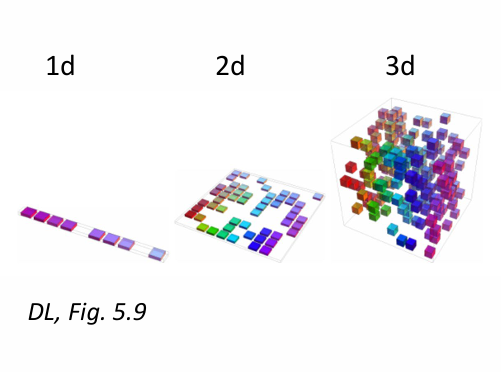
\includegraphics[width=0.75\linewidth]{Images/curse-dimensionality.png}
    \caption{Curse of High Dimensionality: Sample density decreases if not mitigated by exponentially more samples}
\end{figure}

\defn{Local Constancy and Smoothness}{
    For good generalization we guide by some form of prior knowledge.
    Very popular is the smoothness (local constancy) prior:
    \begin{equation*}
        f*(x) \approx f*(x+\epsilon)
    \end{equation*}
    The function should not change much in small neighborhood \(\epsilon\).
    Many classical ml schemes are based on this (KNN, Trees, SVM) and tend to fail in more complex tasks.
    \textbf{Deep learning introduces additional priors.}
}

\begin{figure}[H]
    \centering
    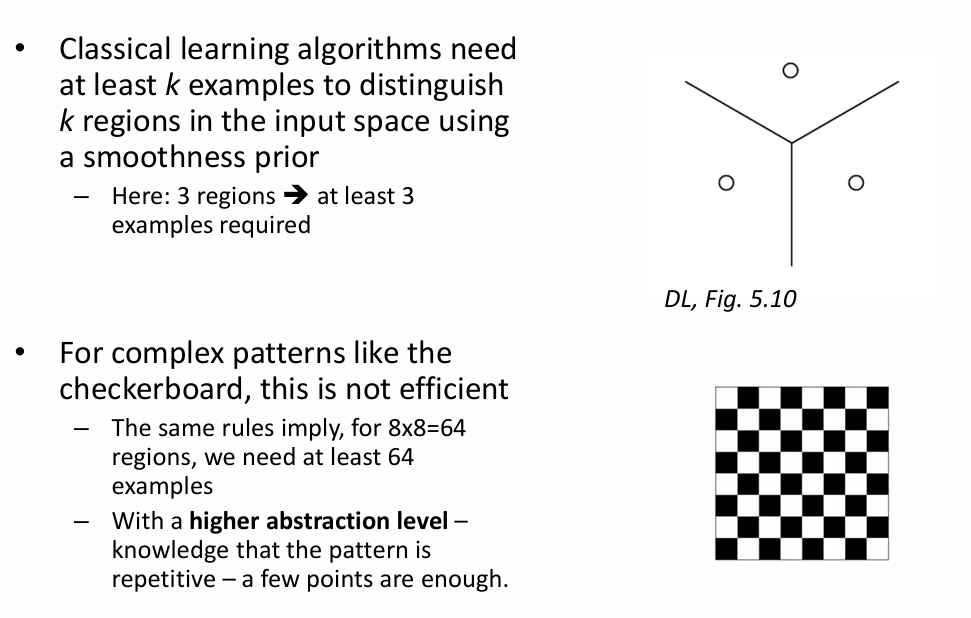
\includegraphics[width=0.75\linewidth]{Images/local-constancy.png}
    \caption{Local Constancy}
\end{figure}

\subsection{Local Constancy in Deep Learning}
The \textbf{core assumption} in deep learning is \textbf{composition of factors}.
We assume the data was generated hierarchically over several levels by the composition of factors.

These (mild) assumptions allow for an exponential relationship between
the number of training examples and the number of regions that can be distinguished.

\begin{figure}[H]
    \centering
    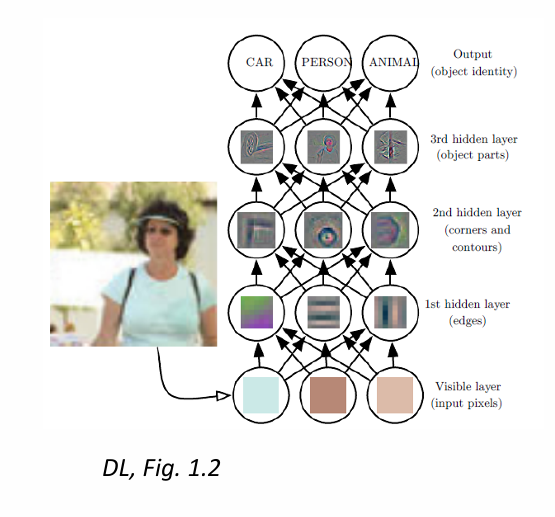
\includegraphics[width=0.75\linewidth]{Images/composition-factors.png}
    \caption{Composition of Factors: We assume exponential hierarchical relationships between the training examples}
\end{figure}

\defn{Manifold Learning}{
    A manifold is a set of points 
    associated with a \textbf{neighborhood} 
    around each point or also a smaller dimensional region
    in a higher dimensional space.
    From any given point, the manifold 
    locally appears to be a Euclidean space.
    The idea of a manifold is, that the 
    connected set of points can be 
    approximated well by considering 
    only a small number of dimensions, 
    embedded in a higher-dimensional space.
    Many problems seem arbitrarily 
    complex, if the scheme needs to 
    learn functions with variations 
    across all dimensions. In manifold learning, this is simplified 
    by assuming that\textbf{ interesting inputs 
    must lie along manifolds}. Hence 
    most inputs are not valid inputs.
}

\begin{figure}[H]
    \centering
    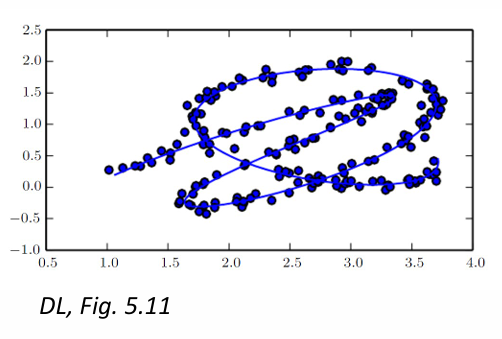
\includegraphics[width=0.75\linewidth]{Images/manifold-example-1.png}
    \caption{Manifold Example: Interesting points follow a lower dimensional manifold in higher dimensional space.}
\end{figure}

\begin{figure}[H]
    \centering
    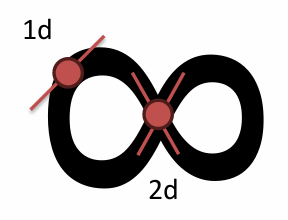
\includegraphics[width=0.25\linewidth]{Images/manifold-example-2.png}
    \caption{Manifold Example: In machine learning, the dimensionality of the manifold is 
    allowed to vary from one point to another. This for example happens at an intersection.}
\end{figure}

The assumption that the data lies along a low-dimensional manifold 
may not always be correct or useful.
However for many tasks the assumpation may seem to hold or be atleast useful.

\begin{figure}[H]
    \centering
    \includegraphics[width=1\linewidth]{Images/manifold-example-3.png}
\end{figure}
\begin{figure}[H]
    \centering
    \includegraphics[width=0.75\linewidth]{Images/manifold-example-4.png}
\end{figure}

\section{Deep Feedforward Networks}
Synonyms:
\begin{itemize}
    \item Deep Feedforward Network
    \item Feedforward Neural Network
    \item Fully-Connected Neural Network
    \item Dense Neural Network
    \item Multilayer Perceptron (MLP)
        \begin{itemize}
            \item Historically it was first a perceptron modelled after biological neurons.
            \item Stacked together they form a MLP, hence basically the same as a Deep Feedforward Network
        \end{itemize}
\end{itemize}
Dense or fully connected refers to networks in which each neuron in the layers are interconnected to each previous neurons.

\defn{DFN Core Concept}{
    Core idea: represent functions 
    with higher and higher 
    complexity by adding more and 
    more layers.

    Called feedforward because 
    information flows from input to 
    output, hence No loops / cycles also a directed acyclic graph (DAG).

    We approximate some unknown function \(f*(x)\) with:
    \begin{equation}
        y = f(x,\theta)
    \end{equation}
    Using function composition (chaining of vector functions):
    \begin{equation}
        f(x) = f^{(3)}(f^{(2)}(f^{(1)}(x)))
    \end{equation}

    Instead of interpreting the layers as 
    vector valued functions, each layer 
    can be considered of consisting of an 
    array of (mathematical) neurons.

    The output of a neuron is usually called an 
    activation and hence the function these 
    neurons calculate are usually called 
    activation functions
}

\subsection{Capacity of classical ML (XOR-Problem)}
Linear models have a very limited capacity.
Very famously linear models cannot solve the simple XOR problem.

Linear models can be extended by 
applying a nonlinear function to x 
and then applying a linear model to 
the transformed x:
\begin{equation}
    \phi(x)
\end{equation}
The problem now boils down to finding such a mapping:
\begin{enumerate}
    \item Manually engineer \(\phi(x)\)
        \begin{itemize}
            \item Classical approach
            \item High Effort
            \item Does not work well in many domain e.g due to unknown structures
        \end{itemize}
    \item User a very generic \(\phi(x)\)
        \begin{itemize}
            \item E.g SVM with RBF-Kernel
            \item Often not powerfull (complex) enough
        \end{itemize}
    \item Learn \(\phi(x)\) itself
        \begin{itemize}
            \item Done in Deep Learning
        \end{itemize}
\end{enumerate}

\subsubsection{XOR-Problem}
\defn{XOR Linear Regression}{
    When trying to solve the XOR-Problem using:
    \begin{equation*}
        f(x,w,b) = x^T w + b
    \end{equation*}
    and cost function:
    \begin{equation*}
        J(\theta) = \frac{1}{4} \sum_{x \in \mathbb{X}} (f*(x) - f(x;\theta))^2
    \end{equation*}
    Solving optimaly for \(\theta\) results in:
    \begin{equation*}
        w = 0, b = \frac{1}{2}
    \end{equation*}
    Hence the model is not capable to represent this function.
}

\begin{figure}[H]
    \centering
    \includegraphics[width=0.75\linewidth]{Images/xorproblem.png}
    \caption{XOR-Problem can be summarized as finding a mapping \(\phi(x)\) so that,
    the problem can be linearly separated. Using linear boundary this is not solvable.}
\end{figure}

\defn{XOR NN}{
    One solution to this problem is, 
    that a network learns a new 
    feature space (representation) 
    where a linear model can solve 
    the problem. See figure \ref{fig:xornn} on page \pageref{fig:xornn}.

    The output layer is still just a linear 
    regression model but now it is 
    applied to the hidden vector h and 
    not to the input vector x.
    This corresponds to a linear regression applied to a transformation:
    \begin{equation*}
        h = \phi(x)
    \end{equation*}

    \textbf{Typically}, the activation function is an 
    element-wise function, hence each 
    output hi is independent.
    \textbf{Hence, we don't need Jacobians to 
    calculate the gradient!}
}

\begin{figure}[H]
    \centering
    \includegraphics[width=0.5\linewidth]{Images/xornn.png}
    \caption{NN Model Architecture that is able to solve XOR. Only one layer is needed
    since the non-linear activation function is able to map the problem so that its linearly seperatable.}
    \label{fig:xornn}
\end{figure}

\begin{figure}[H]
    \centering
    \includegraphics[width=0.75\linewidth]{Images/xornnexample.png}
    \caption{We can manualy evaluate the simple NN for the NN problem.}
\end{figure}
\begin{figure}[H]
    \centering
    \includegraphics[width=0.75\linewidth]{Images/xornnexample-2.png}
    \caption{When applying the nonlinear function (RELU) the magic happens:
    Negative values are mapped to zero, this creates a new data representation that is linearly seperable.
    If we now in the final step find a linear boundary using a linear model the problem is solvable.}
\end{figure}

\subsection{Gradient Based Learning}
\begin{itemize}
    \item We typically use a negative log lieklihood
    \item NN have loss functions which are \textbf{not convex}
        \begin{itemize}
            \item Hence GD will probably not find a global minimum
            \item Wordks well in practice
            \item Initialization of weights and biases is of major importance.
        \end{itemize}
\end{itemize}

\defn{Gradient Based Learning}{
   Use gradient method to minimize:
   \begin{equation}
    J(w,b) = -\mathbb{E}_{x \sim \hat{p}_{data}}[\log p_{model}(x)]
   \end{equation}
   We assume an empirical data generating function \(\hat{p}_{data}\).
   And a stochastic model function:
   \begin{equation}
        p_{model}(x) = p(y | x;\theta)
   \end{equation}

   Often the cost function is augmented with a regularization term:
   \begin{equation}
    J(w,b) = \lambda ||w||_2^2 -\mathbb{E}_{x \sim \hat{p}_{data}}[\log p_{model}(x)]
   \end{equation}

   \textbf{Important!}:
   \begin{itemize}
    \item When using gradient-based optimization, it is very important that 
    the gradient does not vanish
        \begin{itemize}
            \item Sigmoid function: narrow space (-1,1) and g=0 everywhere else
            \item Relu: g=0 if <0
            \item Leaky Relu introduces gradient by multiplying by small value if <0.
        \end{itemize}
    \item Negative Log-Likelihood has numerical advantages:
        \begin{itemize}
            \item output units involve often an exponential function.
            which will saturate, when the argument is very negative.
            Log function undoes the exp function, hence this allows for progress
        \end{itemize}
   \end{itemize}
}

\begin{figure}[H]
    \centering
    \includegraphics[width=1\linewidth]{Images/outputunit.png}
    \caption{Most used output units}
\end{figure}

\defn{Quantative}{
    \begin{equation}
        p(y|x) = N(y;(W^T h + b),I)
    \end{equation}
    In this case, the 
    Maximum Likelihood is equivalent 
    to minimizing the MSE.
    if the variance is not 
    constant, a different method must 
    be used. For example, the variance can also be learned.
}

\defn{Bernoulli Output}{
    \begin{equation}
        \phi = P(y=1 | x)
    \end{equation}
    he parameter \(\phi\) of a Bernoulli 
    must be between 0 and 1 Otherwise, it is not a valid 
    probability.

    We could use:
    \begin{equation*}
        P(y=1|x) = max \{0, min \{ 1, w^T h + b \}\}
    \end{equation*}
    But at the boundaries the optimization does not work because g=0.
    Thus we use the sigmoid:
    \begin{equation}
        P(y=1|x) = \sigma(w^T h + b)
    \end{equation}
    If we take this further we can show \ref{fig:sigmoidtosoftmax} on page \pageref{fig:sigmoidtosoftmax}:
    \begin{equation}
        \begin{split}
            P(y|z) &= \sigma((2y-1)z) \\
            J(\theta) &= \xi((1-2y)z)
        \end{split}
    \end{equation}
    Where \(\xi\) is the \textbf{softmax} function.
}


\begin{figure}[H]
    \centering
    \includegraphics[width=1\linewidth]{Images/sigmoidevidence.png}
    \caption{Reasoning for using the sigmoid function}
\end{figure}


\begin{figure}[H]
    \centering
    \includegraphics[width=0.75\linewidth]{Images/bernoutput.png}
    \caption{Bernoulli Output with Sigmoid results in Softmax}
    \label{fig:sigmoidtosoftmax}
\end{figure}

\begin{figure}[H]
    \centering
    \includegraphics[width=0.75\linewidth]{Images/bernoutput-softmax.png}
    \caption{Bernoulli Output with Sigmoid results in Softmax}
\end{figure}

\defn{Multinoulli}{
    \begin{equation}
        \hat{y}_i = P(y=i|x)
    \end{equation}
    with:
    \begin{equation*}
        z_i = log \hat{P}(y=i | x)
    \end{equation*}
    using:
    \begin{equation}
        \text{softmax}(z)_i = \frac{\exp(z_i)}{\sum_{j} \exp(z_j)}
    \end{equation}
}

\begin{figure}[H]
    \centering
    \includegraphics[width=0.5\linewidth]{Images/commonactivation.png}
    \caption{Common Activation Functions}
\end{figure}

\defn{Universal Approximation Properties and Depth}{
    \begin{itemize}
        \item One can approximate, up to any desired non-zero error all functions using a single sufficiently wide layer 
        \item Mathematically Proven "Multilayer Feedforward Networks are Universal Approximators"
            \begin{itemize}
                \item Regression Problems with linear output unit
                \item Using sigmoid as activation
            \end{itemize}
    \end{itemize}
    theoretically:
    \begin{itemize}
        \item Use sigmoid as activation
        \item Use only 1 layer
        \item Make the hidden layer very wide
    \end{itemize}
    By todays standards this is bad advice:
    \begin{itemize}
        \item Purely theoretical proof
        \item Not guaranteed to ever find a solution
    \end{itemize}

    It was shown that piecewise linear 
    networks (using the abs() as activation 
    function) can represent functions with a 
    number of regions that is exponential in 
    the depth of the network.
}

\begin{figure}[H]
    \centering
    \includegraphics[width=0.5\linewidth]{Images/absfolding.png}
    \caption{Piecewise linear 
    networks using the abs() as activation 
    function can represent functions with a 
    number of regions that is exponential in 
    the depth of the network, by folding solution space.}
\end{figure}



\end{document}
